\documentclass[12pt]{report}
\usepackage{amsthm}
\usepackage{amssymb}
\usepackage{amsmath}
\usepackage{listings}
\usepackage{graphicx}
\usepackage{pgfplots}
\usepackage{float}
\usepackage{xcolor}
\usepackage{hyperref}

\hypersetup{
    colorlinks=true,
    linkcolor=black,
    filecolor=magenta,      
    urlcolor=blue,
    pdftitle={Overleaf Example},
    pdfpagemode=FullScreen,
    }

\setlength{\parindent}{0pt}
\setlength{\parskip}{5pt}
\newcommand{\norm}[1]{\left\|#1\right\|}

\renewcommand\vec{\overrightarrow}

\newtheorem{definition}{Definizione}

\begin{document}

    \title{Parallelizzazione del Problema degli N-Corpi}
    \author{S. Bianco, A. Coppola, F. D'Aprile}
    \date{\today}

    \maketitle
    \tableofcontents
    \newpage

    \chapter{Introduzione}

    \section{Descrizione ed analisi del problema}

    In fisica, il \textbf{problema degli n-corpi} corrisponde al problema inerente alla previsione dei movimenti individuali di un gruppo di $n$ oggetti celesti che interagiscono tra loro gravitazionalmente. Il problema degli n-corpi nella relatività generale è considerevolmente più difficile da risolvere a causa di fattori aggiuntivi come le distorsioni del tempo e dello spazio.
    
    Nella fisica classi, il problema viene informalmente definito come:
    \begin{definition}
        Date le proprietà orbitali quasi-stazionarie (posizione istantanea, velocità e tempo) di un gruppo di n corpi celesti, prevedere le loro forze interattive al fine di prevedere i loro veri movimenti orbitali per tutti i tempi futuri.
    \end{definition}

    In particolare, dati $n$ corpi $b_1, \ldots, b_n$ in uno spazio tridimesionale $\mathbb{R}^3$, siano:
    \begin{itemize}
        \item Gli scalari $m_1, \ldots, m_n$ uguali alle masse dei corpi
        \item I vettori $\vec{p_1}, \ldots, \vec{p_n}$ uguali alle posizioni dei corpi
        \item I vettori $\vec{v_1}, \ldots, \vec{v_n}$ uguali alle velocità dei corpi
    \end{itemize}

    \newpage

    La \textbf{legge di gravità di Newton} afferma che la forza gravitazionale subita in un singolo istante dal corpo $b_i$ da parte di un corpo $b_j$ corrisponde a:
    \[\vec{F_{ij}} = \frac{G m_i m_j}{\norm{\vec{p_j}-\vec{p_i}}^2} \cdot \frac{\vec{p_j}-\vec{p_i}}{\norm{\vec{p_j}-\vec{p_i}}} = \frac{G m_i m_j}{\norm{\vec{p_j}-\vec{p_i}}^3} \cdot (\vec{p_j}-\vec{p_i})\]

    dove $G$ è la \textbf{costante gravitazionale}, ossia $G = 6.67430 \cdot 10^{-11} \frac{\mathrm{N} \cdot m^2}{\mathrm{kg}^2}$ e $\norm{\vec{p_j}-\vec{p_i}}$ è la \textbf{distanza vettoriale} tra $\vec{p_j}$ e $\vec{p_i}$, ossia:
    \[\norm{\vec{p_j}-\vec{p_i}} = \sqrt{(x_j - x_i)^2 + (y_j - y_i)^2 + (z_j - z_i)^2}\]

    Di conseguenza, la somma delle forze subite dal corpo $b_i$ in un singolo istante corrisponde a:
    \[\vec{F_i} = \sum_{\substack{j = 0 \\ j \neq i}}^n \vec{F_{ij}} = \sum_{\substack{j = 0 \\ j \neq i}}^n \frac{G m_i m_j}{\norm{\vec{p_j}-\vec{p_i}}^3} \cdot (\vec{p_j}-\vec{p_i})\]

    Tramite la \textbf{seconda legge di Newton}, invece, sappiamo che la somma delle forze applicate sul corpo $b_i$ ad un instante $t$ corrisponde al prodotto tra la \textit{massa} $m_i$ e la sua \textit{accelerazione} $\vec{a_i}$, ossia:
    \[\vec{F_i} = m_i \vec{a_i}\]
    
    implicando dunque che:
    \[m_i \vec{a_i} =  \sum_{\substack{j = 0 \\ j \neq i}}^n \frac{G m_i m_j}{\norm{\vec{p_j}-\vec{p_i}}^3} \cdot (\vec{p_j}-\vec{p_i}) \iff \vec{a_i} = \sum_{\substack{j = 0 \\ j \neq i}}^n \frac{G m_j}{\norm{\vec{p_j}-\vec{p_i}}^3} \cdot (\vec{p_j}-\vec{p_i})\]

    A questo punto, siano $\vec{v_i}'$ e $\vec{p_i}'$ rispettivamente la velocità e la posizione del corpo $i$ all'iterazione $k+1$ della simulazione. Risulta evidente che:
    \[\vec{v_i}' = \vec{v_i} + \Delta t \cdot \vec{a_i}\]
    \[\vec{p_i}' = \vec{p_i} + \Delta t \cdot \vec{v_i}'\]

    Tuttavia, affinché ogni passo della simulazione risulti \textbf{omogeneo}, è consigliato impostare un valore \textit{non elevato} per $\Delta t$. Poiché tale parametro non influisce sulle performance della simulazione, in quanto la moltiplicazione richieda tempo costante, è stato utilizzato il valore $\Delta t = 1$.
    
    \newpage

    \section{Informazioni sulle statistiche}

    Le statistiche presentate nelle sezioni successive fanno riferimento a \textbf{tempistiche medie} raccolte eseguendo 10 volte ogni simulazione con un range da 1000 a 10000 corpi.
    
    Ogni test è stato eseguito sui seguenti dispositivi:
    \begin{enumerate}
        \item Lenovo IdeaPad 5
        \begin{itemize}
            \item Processore: AMD Ryzen 7 5825U @ 8 cores, 2.0 GHz
            \item Cache per core:
            \begin{itemize}
                \item Cache L1: 512 KB
                \item Cache L2: 4 MB
                \item Cache L3: 16 MB
            \end{itemize}
            \item Memoria: 16 GB DDR4 @ 3200 MHz
        \end{itemize}
        \item MacBook Air M1
        \begin{itemize}
            \item Processore: Apple M1 @ 4 High core, 4 Low core, 2.0 GHz
            \item Cache per core:
            \begin{itemize}
                \item Cache L1: 192+128 MB (High core), 128+64 MB (Low core)
                \item Cache L1: 12 MB (High core), 4 MB (Low core)
            \end{itemize}
            \item Memoria: 16 GB DDR4 @ 3200 MHz
        \end{itemize}
    \end{enumerate}

    Inoltre, le formule utilizzate per calcolare i parametri di \textbf{speed-up} (S) ed \textbf{efficienza} (E) tra le varie versioni sequenziali e parallele sono le seguenti:

    \[S = \frac{T_\text{sequential}}{T_\text{parallel}} \qquad\qquad\qquad E = \frac{S}{p}\]

    dove $p$ è il numero di processori utilizzati

    \chapter{Simulazione tramite metodo esaustivo}

    \section{Implementazione sequenziale}

    All'avvio, il programma procederà con lo \textbf{scansionare il file} contenente i dati dei corpi dato come argomento in input, costruendo un array di struct \texttt{bodies}, ognuno corrispondente ad un corpo. Tali struct sono dotati di tre attributi: un double per la \texttt{massa} del corpo e due \texttt{Vec3D} per la \textit{posizione} e la \textit{velocità} del corpo, dove un \texttt{Vec3D} è un ulteriore struct composto da tre double, uno per ogni coordinata possibile dello spazio tridimensionale (dunque $x,y$ e $z$).

    Tramite l'analisi del capitolo precedente, risulta evidente che l'intera simulazione possa essere implementata tramite tre \textbf{cicli for annidati}:
    \begin{itemize}
        \item Un ciclo esterno che iteri sul numero di passi della simulazione
        \item Un primo ciclo interno che iteri su ognuno degli $n$ corpi della simulazione
        \item Un secondo ciclo interno al primo che calcoli la sommatoria mostrata precedentemente
    \end{itemize}

    \begin{figure}[h]
        \centering
        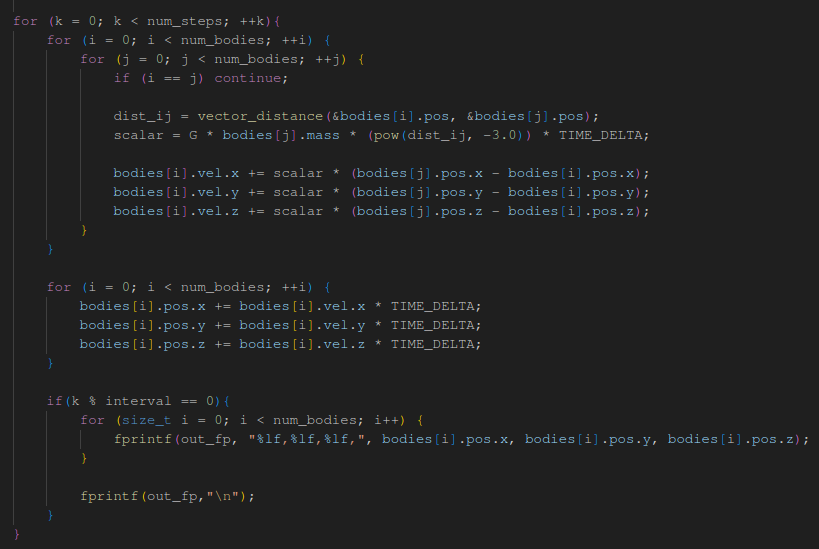
\includegraphics[width=\textwidth]{images/seq_exh_1.png}
        \caption{Screenshot del frammento di codice principale di \texttt{seq\_exh\_1.c}}
        \label{fig:seq_exh_1}
    \end{figure}

    \newpage

    Dati $n$ corpi, eseguendo la simulazione per $k$ passi risulta evidente che il numero complessivo di operazioni eseguite dalla simulazione sia $kn(n-1) = O(kn^2)$.

    Tuttavia, poiché $\norm{\vec{p_i} - \vec{p_j}} = \norm{\vec{p_j} - \vec{p_i}}$, è possibile \textbf{migliorare l'efficienza del programma sequenziale} effettuando nella stessa iterazione i calcoli dell'interazione del corpo $b_i$ con il corpo $b_j$ e viceversa.

    In tal modo, per $n$ corpi e $k$ passi di simulazione, il numero complessivo di iterazioni risulta essere:
    \[k \cdot \sum_{i=0}^n i = k \cdot \frac{n(n+1)}{2}\] 

    \textbf{dimezzando} le iterazioni effettuate, presentando tuttavia comunque un  comportamento asintotico pari a $O(kn^2)$. Inoltre, ogni iterazione effettua quasi il doppio dei calcoli, risparmiando effettivamente solo il ricalcolo della distanza.

    \begin{figure}[H]
        \centering
        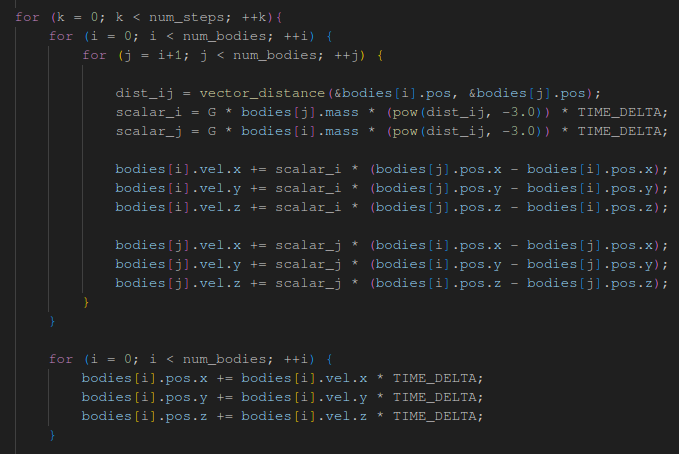
\includegraphics[width=\textwidth]{images/seq_exh_2.png}
        \caption{Screenshot del frammento di codice principale di \texttt{seq\_exh\_2.c}}
        \label{fig:seq_exh_2}
    \end{figure}

    \begin{figure}[H]
        \centering
        
        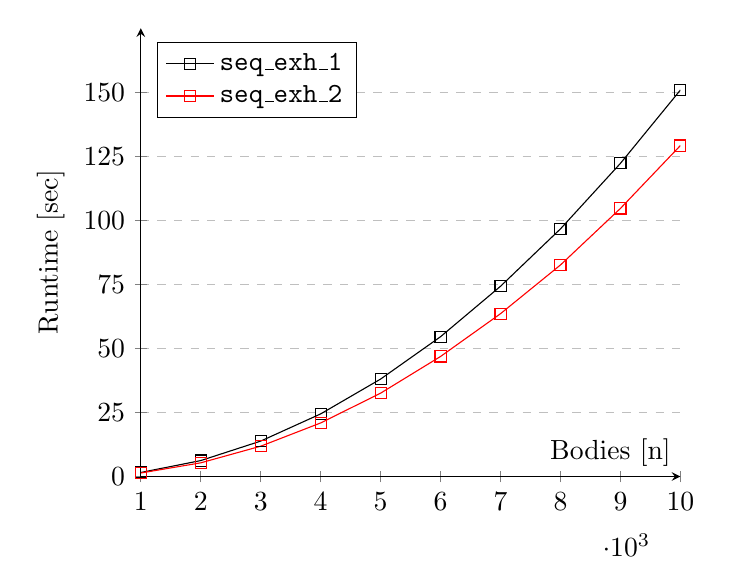
\begin{tikzpicture}
            \begin{axis}[
                axis lines = center,
                hide obscured x ticks=false,
                hide obscured y ticks=false,
                xlabel={Bodies [n]},
                ylabel={Runtime [sec]},
                ylabel near ticks,
                xmin=1000, xmax=10000,
                ymin=0, ymax=175,
                xtick={1000, 2000, 3000, 4000, 5000, 6000, 7000, 8000, 9000, 10000},
                ytick={0, 25, 50, 75, 100, 125, 150},
                legend pos=north west,
                ymajorgrids=true,
                grid style=dashed,
                scaled x ticks= base 10:-3
            ]
            
            \addplot[
                color=black,
                mark=square,
                ]
                coordinates {
                (1000, 1.588418460)
                (2000, 6.230024672)
                (3000, 13.835473919)
                (4000, 24.445233798)
                (5000, 38.049215651)
                (6000, 54.591586947)
                (7000, 74.272990847)
                (8000, 96.675407171)
                (9000, 122.254725814)
                (10000, 150.870804667)
                };

            \addplot[
                color=red,
                mark=square,
                ]
                coordinates {
                (1000, 1.379133129)
                (2000, 5.347227907)
                (3000, 11.842611241)
                (4000, 20.921516943)
                (5000, 32.545111585)
                (6000, 46.869289804)
                (7000, 63.570259547)
                (8000, 82.589148092)
                (9000, 104.659138370)
                (10000, 129.205970407)
                };

            \legend{\texttt{seq\_exh\_1},\texttt{seq\_exh\_2}}
            \end{axis}
        \end{tikzpicture}

        \caption{Confronto delle performance di \texttt{seq\_exh\_1} e \texttt{seq\_exh\_2} su 100 passi di simulazione da 1000 a 10000 corpi (Lenovo IdeaPad 5)}
        \label{fig:seq_exh_table_ip5}
    \end{figure}

    \begin{figure}[H]
        \centering
        
        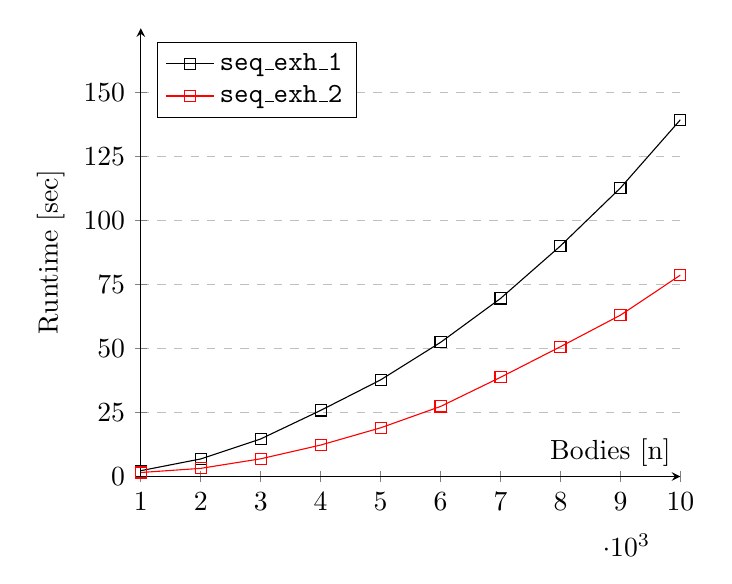
\begin{tikzpicture}
            \begin{axis}[
                axis lines = center,
                hide obscured x ticks=false,
                hide obscured y ticks=false,
                xlabel={Bodies [n]},
                ylabel={Runtime [sec]},
                ylabel near ticks,
                xmin=1000, xmax=10000,
                ymin=0, ymax=175,
                xtick={1000, 2000, 3000, 4000, 5000, 6000, 7000, 8000, 9000, 10000},
                ytick={0, 25, 50, 75, 100, 125, 150},
                legend pos=north west,
                ymajorgrids=true,
                grid style=dashed,
                scaled x ticks= base 10:-3
            ]
            
            \addplot[
                color=black,
                mark=square,
                ]
                coordinates {
                (1000, 2.29056454)
                (2000, 6.86578417)
                (3000, 14.67731190)
                (4000, 25.80976057)
                (5000, 37.72510433)
                (6000, 52.36848545)
                (7000, 69.51298285)
                (8000, 90.02810717)
                (9000, 112.65391874)
                (10000, 139.26667118)
                };

            \addplot[
                color=red,
                mark=square,
                ]
                coordinates {
                (1000, 1.57225609)
                (2000, 3.19314194)
                (3000, 6.92466593)
                (4000, 12.28637600)
                (5000, 19.01857376)
                (6000, 27.35763597)
                (7000, 38.73442936)
                (8000, 50.68782282)
                (9000, 62.99114656)
                (10000, 78.62022018)
                };

            \legend{\texttt{seq\_exh\_1},\texttt{seq\_exh\_2}}
            \end{axis}
        \end{tikzpicture}

        \caption{Confronto delle performance di \texttt{seq\_exh\_1} e \texttt{seq\_exh\_2} su 100 passi di simulazione da 1000 a 10000 corpi (MacBook Air M1)}
        \label{fig:seq_exh_table_m1}
    \end{figure}
    
    \quad

    \section{Parallelizzazione tramite OpenMP}

    \subsection{Approccio naïve}

    Tramite la libreria \textbf{OpenMP}, il codice mostrato nella sezione precedente può facilmente essere parallelizzato applicando la direttiva \texttt{\#pragma omp for} sul primo \textit{ciclo for} interno (ossia quello che itera sui corpi), in modo che ognuno dei $p$ thread su cui viene parallelizzato il ciclo vada a lavorare con $\mathbf{\frac{n}{p}}$ \textbf{corpi}.

    Tuttavia, tale parallelizzazione \underline{non} può essere applicata sulla seconda versione del programma sequenziale (ossia \texttt{seq\_exh\_2}), poiché potrebbe verificarsi una \textbf{race condition} nell'aggiornare la velocità del corpo $b_j$:
    
    \begin{itemize}
        \item Supponiamo che un primo thread stia calcolando l'interazione tra il corpo $b_i$ e $b_j$, aggiornando le velocità di quest'ultimi e che un secondo thread stia calcolando l'interazione tra il corpo $b_j$ con un altro corpo $b_x$, aggiornando la velocità di quest'ultimi
        \item Se i due thread eseguono l'aggiornamento della velocità di $b_j$ simultaneamente, una delle due modifiche verrebbe persa
    \end{itemize}

    Consideriamo ora il \textit{ciclo for} che si occupa della \textit{scrittura dell'output}. Parallelizzando tale ciclo tramite la direttiva \texttt{\#pragma omp for}, i vari thread potrebbero accedere al file simultaneamente, scrivendo  

    Di conseguenza, solo il calcolo delle velocità della versione \texttt{seq\_exh\_1} risulta essere parallelizzabile. Per tanto, i \textbf{confronti statistici} effettuati nelle sezioni successive verranno effettuati \underline{solo} con la versione \texttt{seq\_exh\_1}.

    \begin{figure}[H]
        \centering
        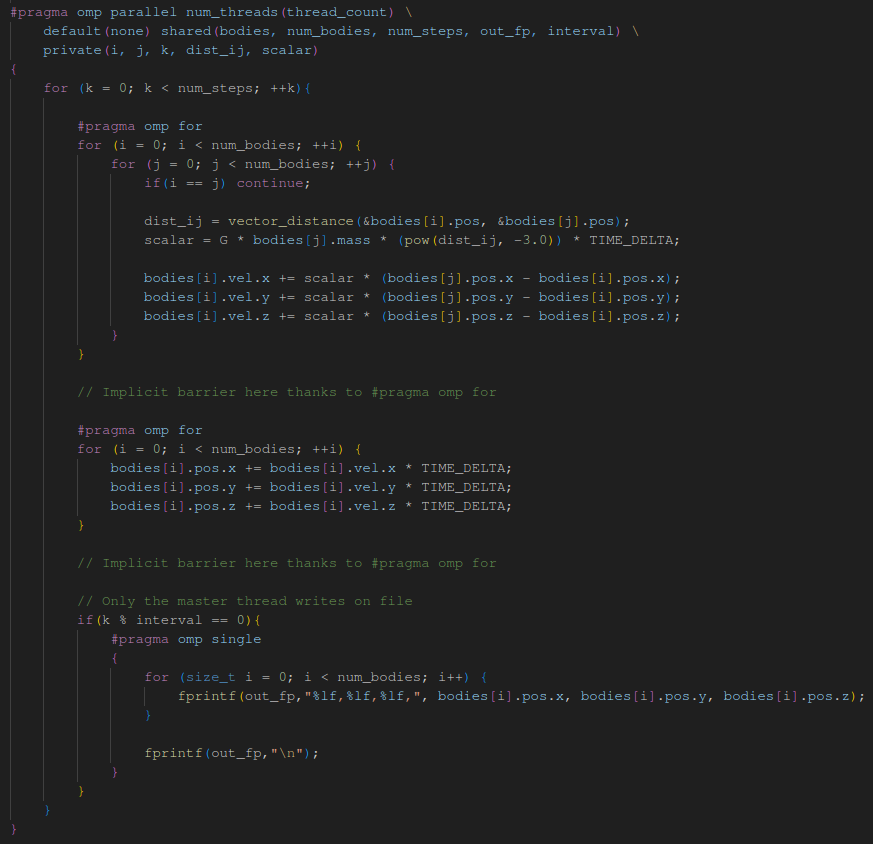
\includegraphics[width=\textwidth]{images/omp_exh_1.png}
        \caption{Screenshot del frammento di codice principale di \texttt{omp\_exh\_1.c}}
        \label{fig:omp_exh_1}
    \end{figure}

    \begin{figure}[H]
        \centering
        
        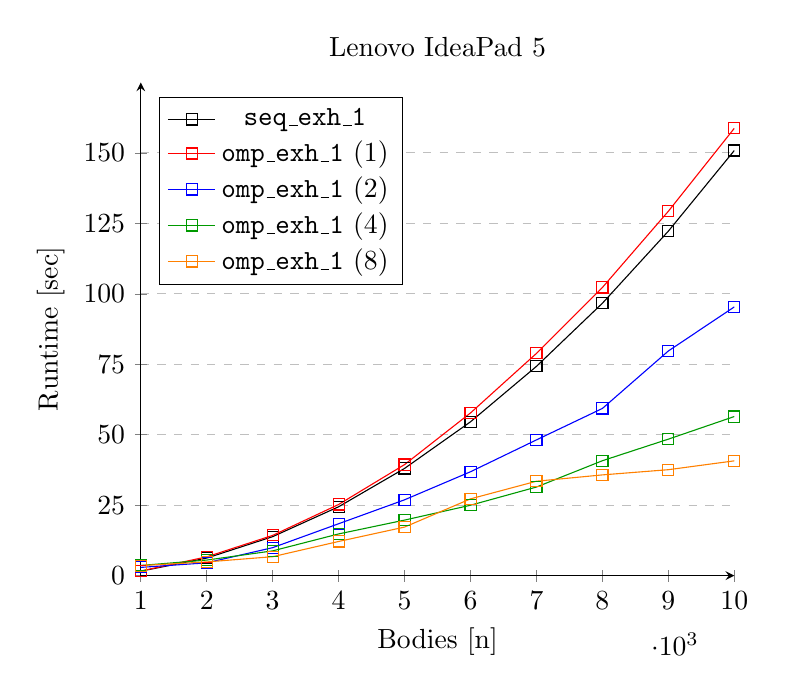
\begin{tikzpicture}
            \begin{axis}[
                axis lines = center,
                hide obscured x ticks=false,
                hide obscured y ticks=false,
                xlabel={Bodies [n]},
                ylabel={Runtime [sec]},
                ylabel near ticks,
                xlabel near ticks,
                xmin=1000, xmax=10000,
                ymin=0, ymax=175,
                xtick={1000, 2000, 3000, 4000, 5000, 6000, 7000, 8000, 9000, 10000},
                ytick={0, 25, 50, 75, 100, 125, 150},
                legend pos=north west,
                ymajorgrids=true,
                grid style=dashed,
                scaled x ticks= base 10:-3,
                scale=1.1,
                title=Lenovo IdeaPad 5
            ]
            
            \addplot[
                color=black,
                mark=square,
                ]
                coordinates {
                (1000, 1.588418460)
                (2000, 6.230024672)
                (3000, 13.835473919)
                (4000, 24.445233798)
                (5000, 38.049215651)
                (6000, 54.591586947)
                (7000, 74.272990847)
                (8000, 96.675407171)
                (9000, 122.254725814)
                (10000, 150.870804667)
                };

            \addplot[
                color=red,
                mark=square,
                ]
                coordinates {
                (1000, 1.645367622)
                (2000, 6.667968750)
                (3000, 14.286896229)
                (4000, 25.254158497)
                (5000, 39.410335541)
                (6000, 57.736707687)
                (7000, 78.864385128)
                (8000, 102.263175011)
                (9000, 129.314517498)
                (10000, 158.753837109)
                };
            
            \addplot[
                color=blue,
                mark=square,
                ]
                coordinates {
                (1000, 2.929732323)
                (2000, 4.547196865)
                (3000, 9.932800293)
                (4000, 18.417196751)
                (5000, 26.913431644)
                (6000, 36.869939327)
                (7000, 48.173758507)
                (8000, 59.336232662)
                (9000, 79.735921860)
                (10000, 95.364573956)
                };

            \addplot[
                color=green!60!black,
                mark=square,
                ]
                coordinates {
                (1000, 3.615668297)
                (2000, 5.525482655)
                (3000, 8.790148258)
                (4000, 14.802278519)
                (5000, 19.71200847)
                (6000, 24.986462593)
                (7000, 31.448183537)
                (8000, 40.785578728)
                (9000, 48.439564705)
                (10000, 56.463528633)
                };

            
            \addplot[
                color=orange,
                mark=square,
                ]
                coordinates {
                (1000, 3.565580845)
                (2000, 4.867418766)
                (3000, 6.723211765)
                (4000, 12.125409603)
                (5000, 17.234317303)
                (6000, 27.247138977)
                (7000, 33.505674839)
                (8000, 35.752236843)
                (9000, 37.599022388)
                (10000, 40.738933086)
                };
    

            \legend{\texttt{seq\_exh\_1},\texttt{omp\_exh\_1} (1), \texttt{omp\_exh\_1} (2), \texttt{omp\_exh\_1} (4), \texttt{omp\_exh\_1} (8), }
            \end{axis}
        \end{tikzpicture}

        \quad 
        
        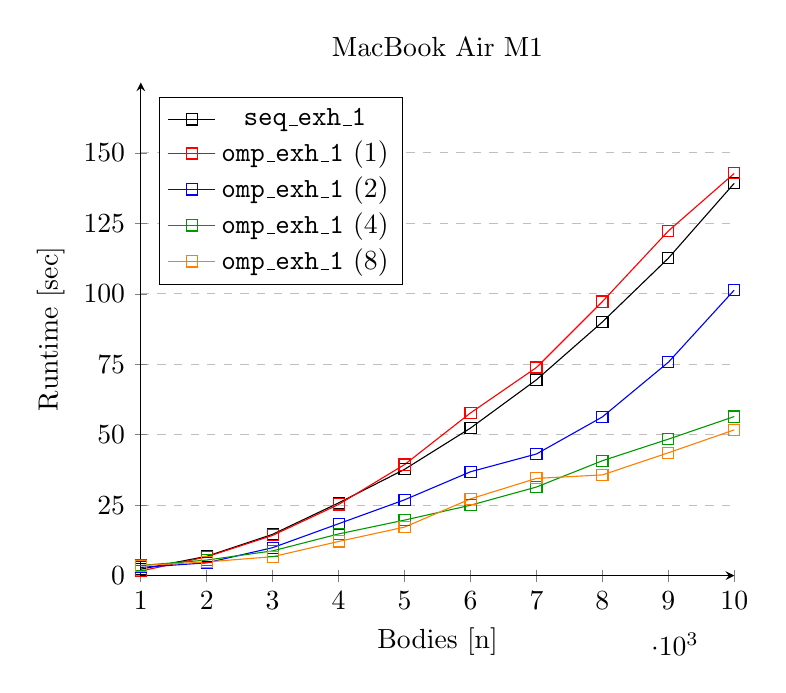
\begin{tikzpicture}
            \begin{axis}[
                axis lines = center,
                hide obscured x ticks=false,
                hide obscured y ticks=false,
                xlabel={Bodies [n]},
                ylabel={Runtime [sec]},
                ylabel near ticks,
                xlabel near ticks,
                xmin=1000, xmax=10000,
                ymin=0, ymax=175,
                xtick={1000, 2000, 3000, 4000, 5000, 6000, 7000, 8000, 9000, 10000},
                ytick={0, 25, 50, 75, 100, 125, 150},
                legend pos=north west,
                ymajorgrids=true,
                grid style=dashed,
                scaled x ticks= base 10:-3,
                scale=1.1,
                title=MacBook Air M1
            ]
            
            \addplot[
                color=black,
                mark=square,
                ]
                coordinates {
                (1000, 2.29056454)
                (2000, 6.86578417)
                (3000, 14.67731190)
                (4000, 25.80976057)
                (5000, 37.72510433)
                (6000, 52.36848545)
                (7000, 69.51298285)
                (8000, 90.02810717)
                (9000, 112.65391874)
                (10000, 139.26667118)
                };

            \addplot[
                color=red,
                mark=square,
                ]
                coordinates {
                (1000, 1.645367622)
                (2000, 6.667968750)
                (3000, 14.286896229)
                (4000, 25.254158497)
                (5000, 39.410335541)
                (6000, 57.736707687)
                (7000, 73.864385128)
                (8000, 97.263175011)
                (9000, 122.314517498)
                (10000, 142.753837109)
                };
            
            \addplot[
                color=blue,
                mark=square,
                ]
                coordinates {
                (1000, 2.929732323)
                (2000, 4.547196865)
                (3000, 9.932800293)
                (4000, 18.417196751)
                (5000, 26.913431644)
                (6000, 36.869939327)
                (7000, 43.173758507)
                (8000, 56.336232662)
                (9000, 75.735921860)
                (10000, 101.364573956)
                };

            \addplot[
                color=green!60!black,
                mark=square,
                ]
                coordinates {
                (1000, 3.615668297)
                (2000, 5.525482655)
                (3000, 8.790148258)
                (4000, 14.802278519)
                (5000, 19.71200847)
                (6000, 24.986462593)
                (7000, 31.448183537)
                (8000, 40.785578728)
                (9000, 48.439564705)
                (10000, 56.463528633)
                };

            
            \addplot[
                color=orange,
                mark=square,
                ]
                coordinates {
                (1000, 3.565580845)
                (2000, 4.867418766)
                (3000, 6.723211765)
                (4000, 12.125409603)
                (5000, 17.234317303)
                (6000, 27.247138977)
                (7000, 34.505674839)
                (8000, 35.752236843)
                (9000, 43.599022388)
                (10000, 51.738933086)
                };

            \legend{\texttt{seq\_exh\_1},\texttt{omp\_exh\_1} (1), \texttt{omp\_exh\_1} (2), \texttt{omp\_exh\_1} (4), \texttt{omp\_exh\_1} (8), }
            \end{axis}
        \end{tikzpicture}

        \caption{Confronto delle performance di \texttt{seq\_exh\_1} e \texttt{omp\_exh\_1} su 100 passi di simulazione da 1000 a 10000 corpi. I numeri tra parentesi nella legenda del grafico indicano il numero di thread attivi}
        \label{fig:omp_1_exh_graph}
    \end{figure}

    \newpage

    \subsection{Riduzione del false sharing}

    Nonostante l'incremento delle performance a livello di tempo di esecuzione ottenuto con la versione \texttt{omp\_exh\_1}, tale parallelizzazione risulta inefficiente da un punto di vista di \textbf{gestione delle cache}.
    
    Nel secondo \textit{ciclo for} interno, ogni thread legge il proprio valore \texttt{bodies[i].pos} e aggiorna i valori del proprio valore \texttt{bodies[i].vel}, entrambi dettati dal proprio indice attuale \texttt{i}.

    \begin{figure}[H]
        \centering
        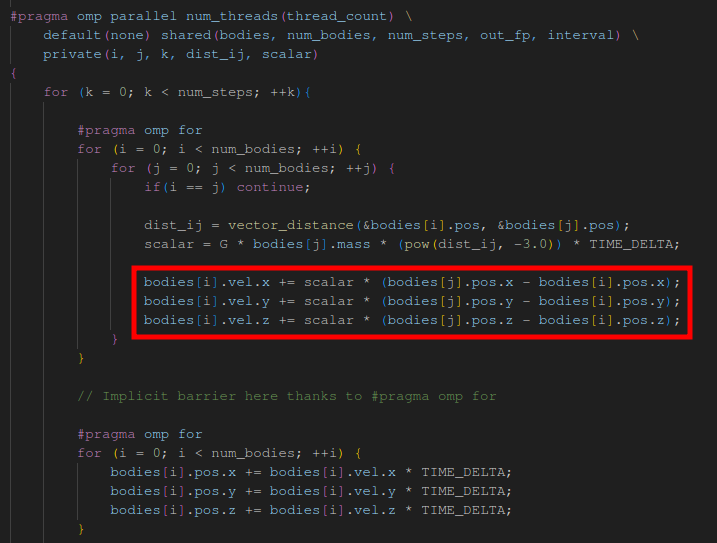
\includegraphics[width=\textwidth]{images/omp_exh_1_false_sharing.png}
        \caption{Screenshot del frammento di codice di interesse di \texttt{omp\_exh\_1.c}}
        \label{fig:omp_exh_1_false_sharing}
    \end{figure}

    Poiché all'interno dello struct \texttt{bodies} i due attributi \texttt{vel} e \texttt{pos} risultano essere memorizzati sequenzialmente all'interno della memoria (ossia accanto), ogni volta che il valore di \texttt{bodies[i].vel} viene modificato da un thread e successivamente un altro thread accede a \texttt{bodies[j].pos}, se $i = j$ allora l'\textbf{intero} blocco di cache contenente lo struct \texttt{bodies[i]} verrà considerato dal secondo thread come \textit{"sporco"} poiché non sincronizzato con quello del primo thread, dunque potenzialmente scorretto, venendo per tanto \textbf{ricaricato} nonostante il valore di \texttt{bodies[i].pos} non sia stato realmente modificato (\textbf{false sharing tra le cache}). Inoltre, considerando il fatto che anche l'array \texttt{bodies} memorizzi i vari corpi sequenzialmente, il false sharing si verifica potenzialmente ad ogni aggiornamento di un corpo.
    

    Introducendo una \textbf{variabile di supporto} che funga da \textit{"accumulatore"} per l'incremento della velocità del corpo attualmente computato, è possibile \textbf{azzerare il false sharing}
    
    \begin{figure}[H]
        \centering
        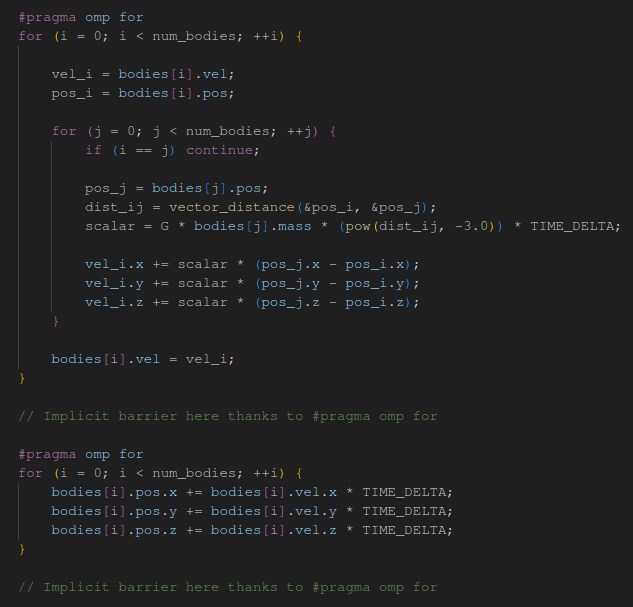
\includegraphics[width=\textwidth]{images/omp_exh_2.png}
        \caption{Screenshot del frammento di codice principale di \texttt{omp\_exh\_2.c}}
        \label{fig:omp_exh_2}
    \end{figure}
    
    \begin{figure}[H]
        \centering
        
        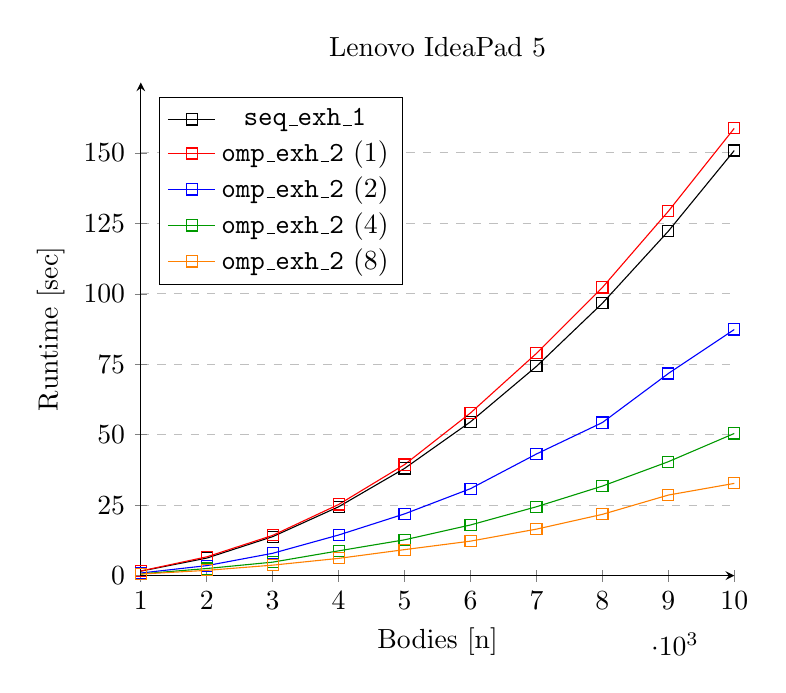
\begin{tikzpicture}
            \begin{axis}[
                axis lines = center,
                hide obscured x ticks=false,
                hide obscured y ticks=false,
                xlabel={Bodies [n]},
                ylabel={Runtime [sec]},
                ylabel near ticks,
                xlabel near ticks,
                xmin=1000, xmax=10000,
                ymin=0, ymax=175,
                xtick={1000, 2000, 3000, 4000, 5000, 6000, 7000, 8000, 9000, 10000},
                ytick={0, 25, 50, 75, 100, 125, 150},
                legend pos=north west,
                ymajorgrids=true,
                grid style=dashed,
                scaled x ticks= base 10:-3,
                scale=1.1,
                title=Lenovo IdeaPad 5
            ]
            
            \addplot[
                color=black,
                mark=square,
                ]
                coordinates {
                (1000, 1.588418460)
                (2000, 6.230024672)
                (3000, 13.835473919)
                (4000, 24.445233798)
                (5000, 38.049215651)
                (6000, 54.591586947)
                (7000, 74.272990847)
                (8000, 96.675407171)
                (9000, 122.254725814)
                (10000, 150.870804667)
                };

            \addplot[
                color=red,
                mark=square,
                ]
                coordinates {
                (1000, 1.645367622)
                (2000, 6.667968750)
                (3000, 14.286896229)
                (4000, 25.254158497)
                (5000, 39.410335541)
                (6000, 57.736707687)
                (7000, 78.864385128)
                (8000, 102.263175011)
                (9000, 129.314517498)
                (10000, 158.753837109)
                };
            
            \addplot[
                color=blue,
                mark=square,
                ]
                coordinates {
                (1000, 0.929732323)
                (2000, 3.547196865)
                (3000, 7.932800293)
                (4000, 14.417196751)
                (5000, 21.913431644)
                (6000, 30.869939327)
                (7000, 43.173758507)
                (8000, 54.336232662)
                (9000, 71.735921860)
                (10000, 87.364573956)
                };

            \addplot[
                color=green!60!black,
                mark=square,
                ]
                coordinates {
                (1000, 0.615668297)
                (2000, 2.525482655)
                (3000, 4.790148258)
                (4000, 8.802278519)
                (5000, 12.71200847)
                (6000, 17.986462593)
                (7000, 24.448183537)
                (8000, 31.785578728)
                (9000, 40.439564705)
                (10000, 50.463528633)
                };

            
            \addplot[
                color=orange,
                mark=square,
                ]
                coordinates {
                (1000, 0.565580845)
                (2000, 1.867418766)
                (3000, 3.723211765)
                (4000, 6.125409603)
                (5000, 9.234317303)
                (6000, 12.247138977)
                (7000, 16.505674839)
                (8000, 21.752236843)
                (9000, 28.599022388)
                (10000, 32.738933086)
                };
    

            \legend{\texttt{seq\_exh\_1},\texttt{omp\_exh\_2} (1), \texttt{omp\_exh\_2} (2), \texttt{omp\_exh\_2} (4), \texttt{omp\_exh\_2} (8), }
            \end{axis}
        \end{tikzpicture}

        \quad 
        
        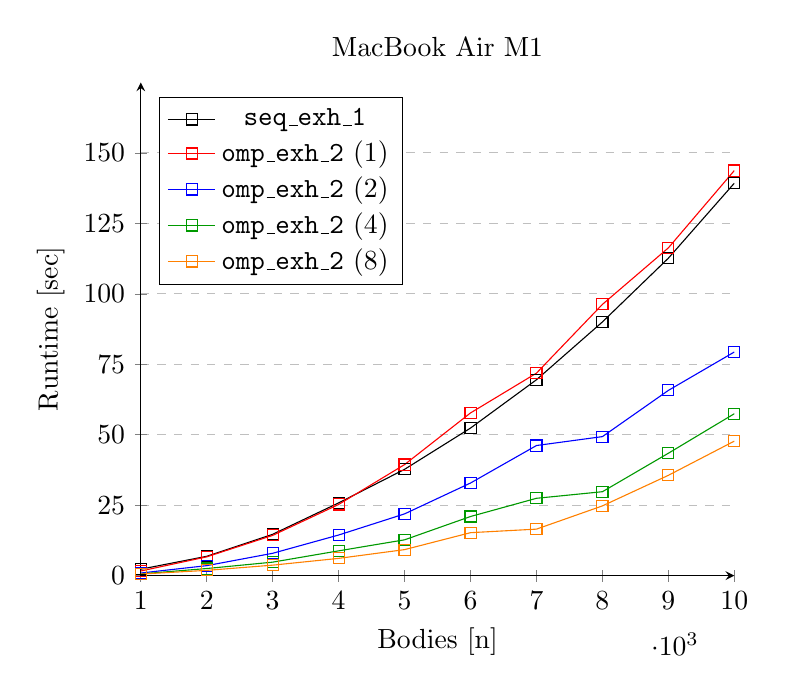
\begin{tikzpicture}
            \begin{axis}[
                axis lines = center,
                hide obscured x ticks=false,
                hide obscured y ticks=false,
                xlabel={Bodies [n]},
                ylabel={Runtime [sec]},
                ylabel near ticks,
                xlabel near ticks,
                xmin=1000, xmax=10000,
                ymin=0, ymax=175,
                xtick={1000, 2000, 3000, 4000, 5000, 6000, 7000, 8000, 9000, 10000},
                ytick={0, 25, 50, 75, 100, 125, 150},
                legend pos=north west,
                ymajorgrids=true,
                grid style=dashed,
                scaled x ticks= base 10:-3,
                scale=1.1,
                title=MacBook Air M1
            ]
            
            \addplot[
                color=black,
                mark=square,
                ]
                coordinates {
                (1000, 2.29056454)
                (2000, 6.86578417)
                (3000, 14.67731190)
                (4000, 25.80976057)
                (5000, 37.72510433)
                (6000, 52.36848545)
                (7000, 69.51298285)
                (8000, 90.02810717)
                (9000, 112.65391874)
                (10000, 139.26667118)
                };

            \addplot[
                color=red,
                mark=square,
                ]
                coordinates {
                (1000, 1.645367622)
                (2000, 6.667968750)
                (3000, 14.286896229)
                (4000, 25.254158497)
                (5000, 39.410335541)
                (6000, 57.736707687)
                (7000, 71.864385128)
                (8000, 96.263175011)
                (9000, 116.314517498)
                (10000, 143.753837109)
                };
            
            \addplot[
                color=blue,
                mark=square,
                ]
                coordinates {
                (1000, 0.929732323)
                (2000, 3.547196865)
                (3000, 7.932800293)
                (4000, 14.417196751)
                (5000, 21.913431644)
                (6000, 32.869939327)
                (7000, 46.173758507)
                (8000, 49.336232662)
                (9000, 65.735921860)
                (10000, 79.364573956)
                };

            \addplot[
                color=green!60!black,
                mark=square,
                ]
                coordinates {
                (1000, 0.615668297)
                (2000, 2.525482655)
                (3000, 4.790148258)
                (4000, 8.802278519)
                (5000, 12.71200847)
                (6000, 20.986462593)
                (7000, 27.448183537)
                (8000, 29.785578728)
                (9000, 43.439564705)
                (10000, 57.463528633)
                };

            
            \addplot[
                color=orange,
                mark=square,
                ]
                coordinates {
                (1000, 0.565580845)
                (2000, 1.867418766)
                (3000, 3.723211765)
                (4000, 6.125409603)
                (5000, 9.234317303)
                (6000, 15.247138977)
                (7000, 16.505674839)
                (8000, 24.752236843)
                (9000, 35.599022388)
                (10000, 47.738933086)
                };

            \legend{\texttt{seq\_exh\_1},\texttt{omp\_exh\_2} (1), \texttt{omp\_exh\_2} (2), \texttt{omp\_exh\_2} (4), \texttt{omp\_exh\_2} (8), }
            \end{axis}
        \end{tikzpicture}

        \caption{Confronto delle performance di \texttt{seq\_exh\_1} e \texttt{omp\_exh\_2} su 100 passi di simulazione da 1000 a 10000 corpi. I numeri tra parentesi nella legenda del grafico indicano il numero di thread attivi}
        \label{fig:omp_2_exh_graph}
    \end{figure}

    \newpage
    
    \subsection{Riduzione dell'overhead di OpenMP}

    Oltre a migliorare la gestione delle cache, è possibile \textbf{minimizzare l'overhead} imposto da OpenMPI. Difatti, nella versione \texttt{omp\_exh\_2}, le due direttive \texttt{\#pragma omp for} vengono maneggiate dal pre-compilatore di OpenMP, venendo sostituite con dei pezzi di codice che vadano a calcolare il modo in cui vengono separati automaticamente gli indici del \textit{ciclo for}.

    Poiché nel programma sono presenti due direttive \texttt{\#pragma omp for} situate all'interno del ciclo esterno che itera $k$ volte sui passaggi della simulazione, tali suddivisioni vengono effettuate per un totale di $2k$ volte.

    Per ridurre tale overhead, è possibile manualmente a priori tale suddivisione prima del ciclo esterno, in modo che ogni thread sappia già su quale pozione di corpi andare ad eseguire i calcoli.
    
    \begin{figure}[H]
        \centering
        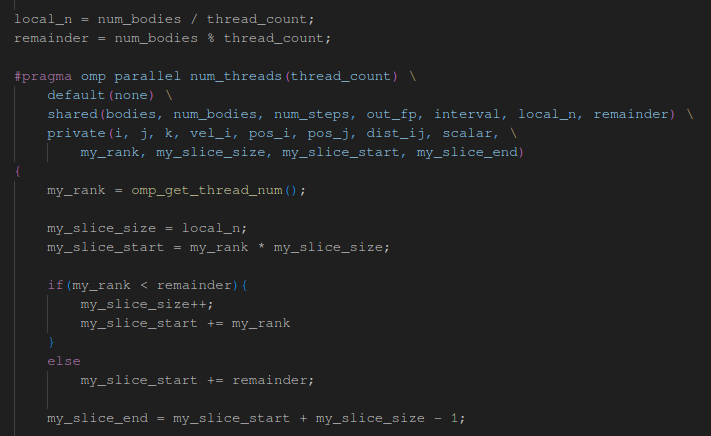
\includegraphics[width=\textwidth]{images/omp_exh_3_1.png}
    \end{figure}

    \begin{figure}[H]
        \centering
        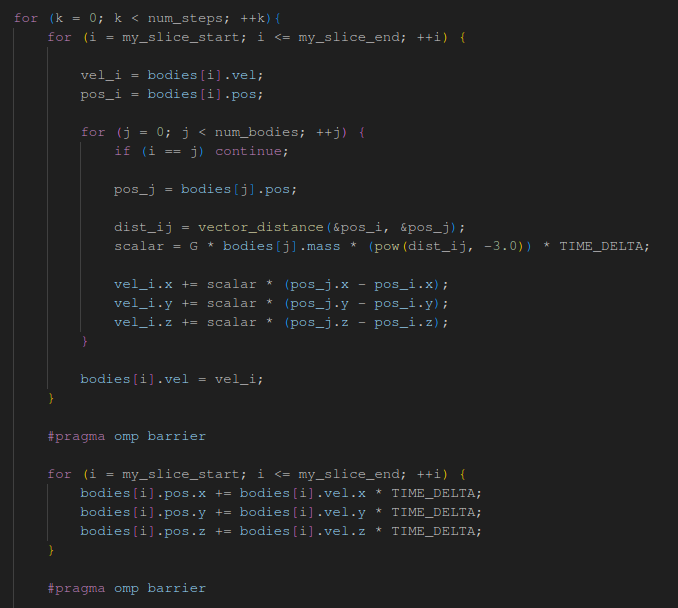
\includegraphics[width=\textwidth]{images/omp_exh_3_2.png}
        \caption{Screenshot del frammento di codice principale di \texttt{omp\_exh\_3.c}}
        \label{fig:omp_exh_3}
    \end{figure}

    Nonostante ciò, tale cambiamento \textbf{influisce poco} sulle prestazioni del programma. Difatti, rispetto alla versione precedente, notiamo come l'overhead \textbf{cresca} nel caso in cui vi siano pochi thread in utilizzo (circa il 15\% più lento), mentre esso \textbf{diminuisca} nel caso in cui vi siano molti thread in utilizzo (circa il 10\% più veloce).

    \begin{figure}[H]
        \centering
        
        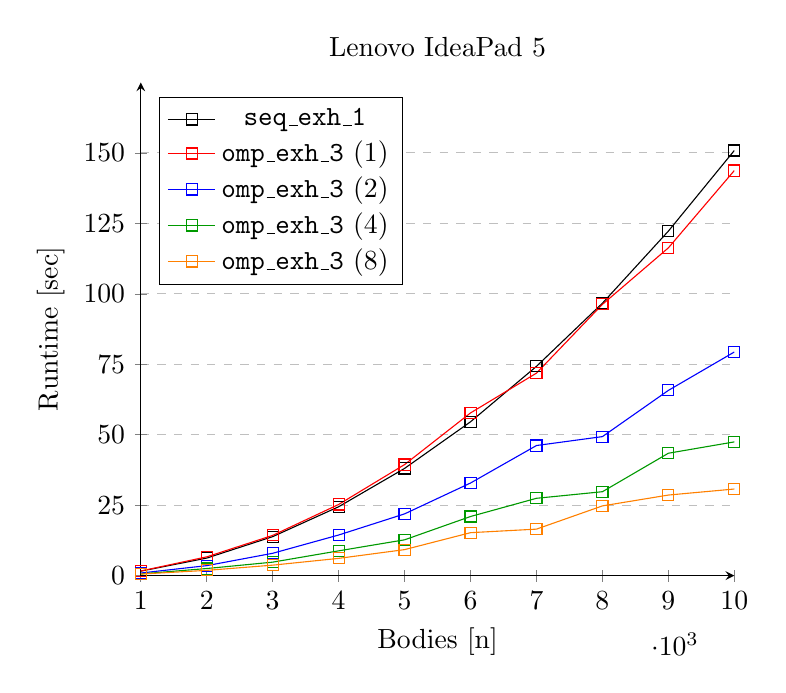
\begin{tikzpicture}
            \begin{axis}[
                axis lines = center,
                hide obscured x ticks=false,
                hide obscured y ticks=false,
                xlabel={Bodies [n]},
                ylabel={Runtime [sec]},
                ylabel near ticks,
                xlabel near ticks,
                xmin=1000, xmax=10000,
                ymin=0, ymax=175,
                xtick={1000, 2000, 3000, 4000, 5000, 6000, 7000, 8000, 9000, 10000},
                ytick={0, 25, 50, 75, 100, 125, 150},
                legend pos=north west,
                ymajorgrids=true,
                grid style=dashed,
                scaled x ticks= base 10:-3,
                scale=1.1,
                title=Lenovo IdeaPad 5
            ]
            
            \addplot[
                color=black,
                mark=square,
                ]
                coordinates {
                (1000, 1.588418460)
                (2000, 6.230024672)
                (3000, 13.835473919)
                (4000, 24.445233798)
                (5000, 38.049215651)
                (6000, 54.591586947)
                (7000, 74.272990847)
                (8000, 96.675407171)
                (9000, 122.254725814)
                (10000, 150.870804667)
                };


                \addplot[
                    color=red,
                    mark=square,
                    ]
                    coordinates {
                    (1000, 1.645367622)
                    (2000, 6.667968750)
                    (3000, 14.286896229)
                    (4000, 25.254158497)
                    (5000, 39.410335541)
                    (6000, 57.736707687)
                    (7000, 71.864385128)
                    (8000, 96.263175011)
                    (9000, 116.314517498)
                    (10000, 143.753837109)
                    };
                
                \addplot[
                    color=blue,
                    mark=square,
                    ]
                    coordinates {
                    (1000, 0.929732323)
                    (2000, 3.547196865)
                    (3000, 7.932800293)
                    (4000, 14.417196751)
                    (5000, 21.913431644)
                    (6000, 32.869939327)
                    (7000, 46.173758507)
                    (8000, 49.336232662)
                    (9000, 65.735921860)
                    (10000, 79.364573956)
                    };
    
                \addplot[
                    color=green!60!black,
                    mark=square,
                    ]
                    coordinates {
                    (1000, 0.615668297)
                    (2000, 2.525482655)
                    (3000, 4.790148258)
                    (4000, 8.802278519)
                    (5000, 12.71200847)
                    (6000, 20.986462593)
                    (7000, 27.448183537)
                    (8000, 29.785578728)
                    (9000, 43.439564705)
                    (10000, 47.463528633)
                    };
    
                
                \addplot[
                    color=orange,
                    mark=square,
                    ]
                    coordinates {
                    (1000, 0.565580845)
                    (2000, 1.867418766)
                    (3000, 3.723211765)
                    (4000, 6.125409603)
                    (5000, 9.234317303)
                    (6000, 15.247138977)
                    (7000, 16.505674839)
                    (8000, 24.752236843)
                    (9000, 28.599022388)
                    (10000, 30.738933086)
                    };

            \legend{\texttt{seq\_exh\_1},\texttt{omp\_exh\_3} (1), \texttt{omp\_exh\_3} (2), \texttt{omp\_exh\_3} (4), \texttt{omp\_exh\_3} (8), }
            \end{axis}
        \end{tikzpicture}

        \quad 
        
        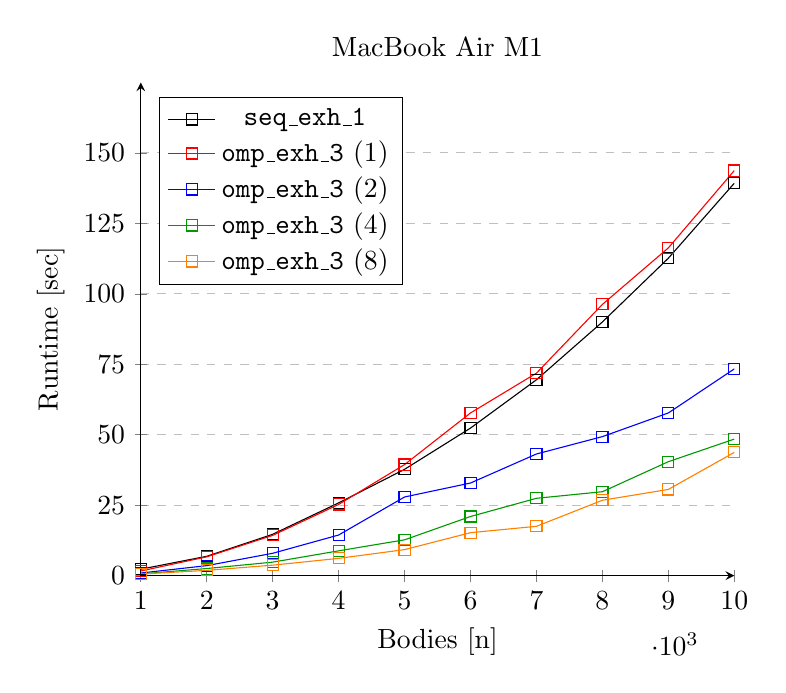
\begin{tikzpicture}
            \begin{axis}[
                axis lines = center,
                hide obscured x ticks=false,
                hide obscured y ticks=false,
                xlabel={Bodies [n]},
                ylabel={Runtime [sec]},
                ylabel near ticks,
                xlabel near ticks,
                xmin=1000, xmax=10000,
                ymin=0, ymax=175,
                xtick={1000, 2000, 3000, 4000, 5000, 6000, 7000, 8000, 9000, 10000},
                ytick={0, 25, 50, 75, 100, 125, 150},
                legend pos=north west,
                ymajorgrids=true,
                grid style=dashed,
                scaled x ticks= base 10:-3,
                scale=1.1,
                title=MacBook Air M1
            ]
            
            \addplot[
                color=black,
                mark=square,
                ]
                coordinates {
                (1000, 2.29056454)
                (2000, 6.86578417)
                (3000, 14.67731190)
                (4000, 25.80976057)
                (5000, 37.72510433)
                (6000, 52.36848545)
                (7000, 69.51298285)
                (8000, 90.02810717)
                (9000, 112.65391874)
                (10000, 139.26667118)
                };

            \addplot[
                color=red,
                mark=square,
                ]
                coordinates {
                (1000, 1.645367622)
                (2000, 6.667968750)
                (3000, 14.286896229)
                (4000, 25.254158497)
                (5000, 39.410335541)
                (6000, 57.736707687)
                (7000, 71.864385128)
                (8000, 96.263175011)
                (9000, 116.314517498)
                (10000, 143.753837109)
                };
            
            \addplot[
                color=blue,
                mark=square,
                ]
                coordinates {
                (1000, 0.929732323)
                (2000, 3.547196865)
                (3000, 7.932800293)
                (4000, 14.417196751)
                (5000, 27.913431644)
                (6000, 32.869939327)
                (7000, 43.173758507)
                (8000, 49.336232662)
                (9000, 57.735921860)
                (10000, 73.364573956)
                };

            \addplot[
                color=green!60!black,
                mark=square,
                ]
                coordinates {
                (1000, 0.615668297)
                (2000, 2.525482655)
                (3000, 4.790148258)
                (4000, 8.802278519)
                (5000, 12.71200847)
                (6000, 20.986462593)
                (7000, 27.448183537)
                (8000, 29.785578728)
                (9000, 40.439564705)
                (10000, 48.463528633)
                };

            
            \addplot[
                color=orange,
                mark=square,
                ]
                coordinates {
                (1000, 0.565580845)
                (2000, 1.867418766)
                (3000, 3.723211765)
                (4000, 6.125409603)
                (5000, 9.234317303)
                (6000, 15.247138977)
                (7000, 17.505674839)
                (8000, 26.752236843)
                (9000, 30.599022388)
                (10000, 43.738933086)
                };

            \legend{\texttt{seq\_exh\_1},\texttt{omp\_exh\_3} (1), \texttt{omp\_exh\_3} (2), \texttt{omp\_exh\_3} (4), \texttt{omp\_exh\_3} (8), }
            \end{axis}
        \end{tikzpicture}

        \caption{Confronto delle performance di \texttt{seq\_exh\_1} e \texttt{omp\_exh\_3} su 100 passi di simulazione da 1000 a 10000 corpi. I numeri tra parentesi nella legenda del grafico indicano il numero di thread attivi}
        \label{fig:omp_3_exh_graph}
    \end{figure}
    \newpage

    Un'ulteriore tentativo di \textit{iper-ottimizzazione} delle performance del programma prevede l'\textbf{eliminazione completa} del false sharing. Difatti, poiché anche i corpi sono memorizzati in modo sequenziale nell'array \texttt{bodies}, potrebbe verificarsi il caso in cui due corpi siano caricati all'interno dello stesso blocco di cache, creando potenzialmente del false sharing.
    
    Per risolvere tale problema, è sufficiente \textit{abbandonare} l'uso dello struct \texttt{bodies} e sostituire l'array \texttt{bodies} con tre array \texttt{masses}, \texttt{positions} e \texttt{velocities}. In tal modo, i valori dello stesso tipo (ossia massa, posizione e velocità) saranno adiacenti a loro, implicando che scrivere e leggere due tipi di valori contemporaneamente non vada a creare false sharing.

    Tuttavia, tale modifica non \textbf{influisce}

    \begin{figure}[H]
        \centering
        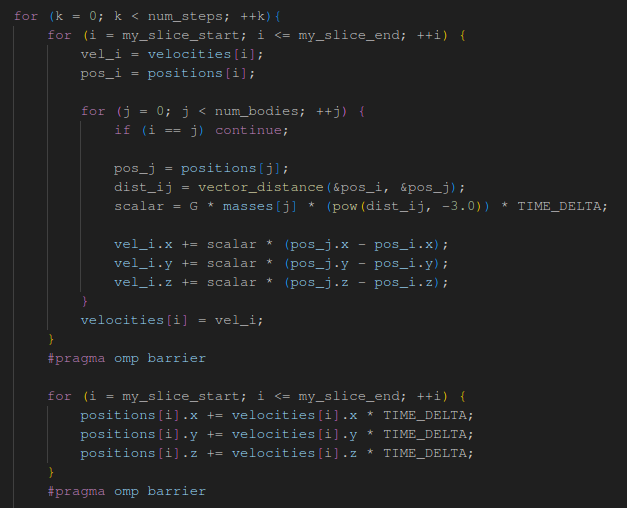
\includegraphics[width=\textwidth]{images/omp_exh_4.png}
        \caption{Screenshot del frammento di codice principale di \texttt{omp\_exh\_4.c}}
        \label{fig:omp_exh_4}
    \end{figure}

    \begin{figure}[H]
        \centering
        
        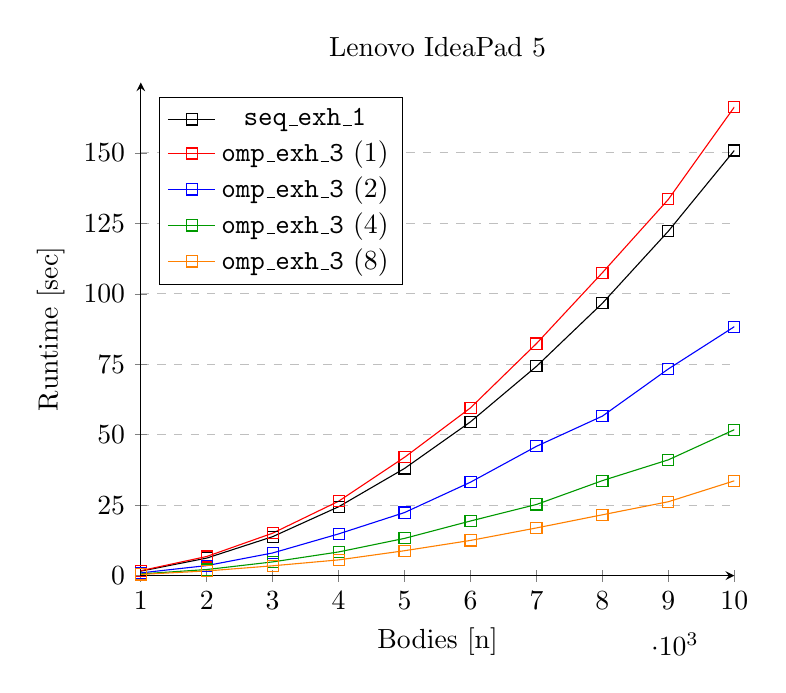
\begin{tikzpicture}
            \begin{axis}[
                axis lines = center,
                hide obscured x ticks=false,
                hide obscured y ticks=false,
                xlabel={Bodies [n]},
                ylabel={Runtime [sec]},
                ylabel near ticks,
                xlabel near ticks,
                xmin=1000, xmax=10000,
                ymin=0, ymax=175,
                xtick={1000, 2000, 3000, 4000, 5000, 6000, 7000, 8000, 9000, 10000},
                ytick={0, 25, 50, 75, 100, 125, 150},
                legend pos=north west,
                ymajorgrids=true,
                grid style=dashed,
                scaled x ticks= base 10:-3,
                scale=1.1,
                title=Lenovo IdeaPad 5
            ]
            
            \addplot[
                color=black,
                mark=square,
                ]
                coordinates {
                (1000, 1.588418460)
                (2000, 6.230024672)
                (3000, 13.835473919)
                (4000, 24.445233798)
                (5000, 38.049215651)
                (6000, 54.591586947)
                (7000, 74.272990847)
                (8000, 96.675407171)
                (9000, 122.254725814)
                (10000, 150.870804667)
                };

            \addplot[
                color=red,
                mark=square,
                ]
                coordinates {
                (1000, 1.750670910)
                (2000, 6.799425602)
                (3000, 15.073948860)
                (4000, 26.405560970)
                (5000, 42.006222725)
                (6000, 59.546832561)
                (7000, 82.359817028)
                (8000, 107.518807411)
                (9000, 133.532767296)
                (10000, 166.285184860)
                };
            
            \addplot[
                color=blue,
                mark=square,
                ]
                coordinates {
                (1000, 0.974502087)
                (2000, 3.566545486)
                (3000, 8.048966885)
                (4000, 14.811261177)
                (5000, 22.396142006)
                (6000, 33.171205521)
                (7000, 45.891497612)
                (8000, 56.616587639)
                (9000, 73.355615139)
                (10000, 88.344113350)
                };

            \addplot[
                color=green!60!black,
                mark=square,
                ]
                coordinates {
                (1000, 0.615656376)
                (2000, 2.165991783)
                (3000, 4.873959541)
                (4000, 8.411749840)
                (5000, 13.226472855)
                (6000, 19.394311905)
                (7000, 25.253199577)
                (8000, 33.725502968)
                (9000, 41.102694988)
                (10000, 51.789970875)
                };

            
            \addplot[
                color=orange,
                mark=square,
                ]
                coordinates {
                (1000, 0.432310581)
                (2000, 1.662023067)
                (3000, 3.493677616)
                (4000, 5.591145515)
                (5000, 8.850440979)
                (6000, 12.494000435)
                (7000, 16.930998802)
                (8000, 21.597300053)
                (9000, 26.231820583)
                (10000, 33.649306774)
                };

            \legend{\texttt{seq\_exh\_1},\texttt{omp\_exh\_3} (1), \texttt{omp\_exh\_3} (2), \texttt{omp\_exh\_3} (4), \texttt{omp\_exh\_3} (8), }
            \end{axis}
        \end{tikzpicture}

        \quad 
        
        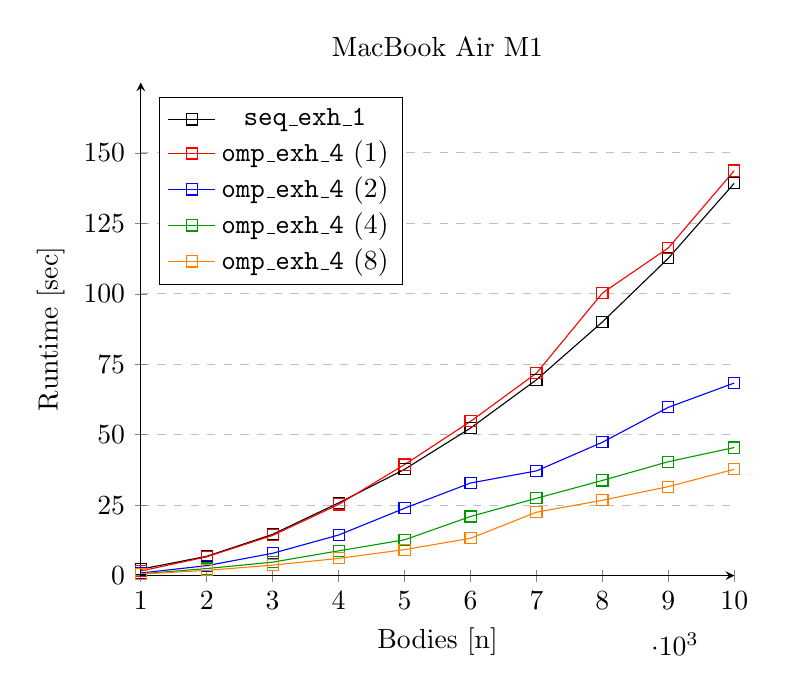
\begin{tikzpicture}
            \begin{axis}[
                axis lines = center,
                hide obscured x ticks=false,
                hide obscured y ticks=false,
                xlabel={Bodies [n]},
                ylabel={Runtime [sec]},
                ylabel near ticks,
                xlabel near ticks,
                xmin=1000, xmax=10000,
                ymin=0, ymax=175,
                xtick={1000, 2000, 3000, 4000, 5000, 6000, 7000, 8000, 9000, 10000},
                ytick={0, 25, 50, 75, 100, 125, 150},
                legend pos=north west,
                ymajorgrids=true,
                grid style=dashed,
                scaled x ticks= base 10:-3,
                scale=1.1,
                title=MacBook Air M1
            ]
            
            \addplot[
                color=black,
                mark=square,
                ]
                coordinates {
                (1000, 2.29056454)
                (2000, 6.86578417)
                (3000, 14.67731190)
                (4000, 25.80976057)
                (5000, 37.72510433)
                (6000, 52.36848545)
                (7000, 69.51298285)
                (8000, 90.02810717)
                (9000, 112.65391874)
                (10000, 139.26667118)
                };

            \addplot[
                color=red,
                mark=square,
                ]
                coordinates {
                (1000, 1.645367622)
                (2000, 6.667968750)
                (3000, 14.286896229)
                (4000, 25.254158497)
                (5000, 39.410335541)
                (6000, 54.736707687)
                (7000, 71.864385128)
                (8000, 100.263175011)
                (9000, 116.314517498)
                (10000, 143.753837109)
                };
            
            \addplot[
                color=blue,
                mark=square,
                ]
                coordinates {
                (1000, 0.929732323)
                (2000, 3.547196865)
                (3000, 7.932800293)
                (4000, 14.417196751)
                (5000, 23.913431644)
                (6000, 32.869939327)
                (7000, 37.173758507)
                (8000, 47.336232662)
                (9000, 59.735921860)
                (10000, 68.364573956)
                };

            \addplot[
                color=green!60!black,
                mark=square,
                ]
                coordinates {
                (1000, 0.615668297)
                (2000, 2.525482655)
                (3000, 4.790148258)
                (4000, 8.802278519)
                (5000, 12.71200847)
                (6000, 20.986462593)
                (7000, 27.448183537)
                (8000, 33.785578728)
                (9000, 40.439564705)
                (10000, 45.463528633)
                };

            
            \addplot[
                color=orange,
                mark=square,
                ]
                coordinates {
                (1000, 0.565580845)
                (2000, 1.867418766)
                (3000, 3.723211765)
                (4000, 6.125409603)
                (5000, 9.234317303)
                (6000, 13.247138977)
                (7000, 22.505674839)
                (8000, 26.752236843)
                (9000, 31.599022388)
                (10000, 37.738933086)
                };

            \legend{\texttt{seq\_exh\_1},\texttt{omp\_exh\_4} (1), \texttt{omp\_exh\_4} (2), \texttt{omp\_exh\_4} (4), \texttt{omp\_exh\_4} (8), }
            \end{axis}
        \end{tikzpicture}

        \caption{Confronto delle performance di \texttt{seq\_exh\_1} e \texttt{omp\_exh\_4} su 100 passi di simulazione da 1000 a 10000 corpi. I numeri tra parentesi nella legenda del grafico indicano il numero di thread attivi}
        \label{fig:omp_4_exh_graph}
    \end{figure}
    
    \newpage

    \newpage

    \section{Parallelizzazione tramite MPI}

    \subsection{Modalità di implementazione}

    Tramite la libreria \textbf{MPI} è possibile parallelizzare il programma creando diversi processi separati (\textbf{memoria distribuita}) che comunicano tramite direttive di scambio di messaggi. Lavorando su zone di memoria separate si evita di incorrere in fenomeni come \textbf{race contion} o \textbf{false sharing} al costo di dover \textit{impostare correttamente gli scambi} tra i processi e degli scambi stessi.

    Un primo approccio per parallelizzare la versione esaustiva prevede la suddivisione dei corpi su cui lavorare tra i processi generati per poi riunire i risultati.
    
    Nel caso particolare in cui si dovesse effettuare \textbf{un solo step} della simulazione, è possibile far sì che un solo processo acquisisca i dati di tutti gli altri processi, restituendoli in output. In tal caso, risulta sufficiente far sì che il \textit{master process} (ossia il processo 0) raccolga i dati calcolati, effettuando una comunicazione All-to-One. Per effettuare una simulazione di \textbf{più passi}, invece, tutti i processi hanno bisogno di conoscere i valori calcolati da ogni altro processo al passo precedente, richiedendo una comunicazione All-to-All.

    Per tanto, ogni processo eseguirà le seguenti fasi:
    \begin{enumerate}
        \item Lettura del file contenente i dati in input
        \item Identificazione dei propri corpi
        \item Calcolo delle nuove posizioni 
        \item Condivisione All-to-All dei risultati
        \item Ripetizione dei passi 3, 4 e 5 per il numero di passi della simulazione 
    \end{enumerate}

    Poiché la lettura del file \textbf{non causa problemi di parallelizzazione} e che tutti i processi hanno bisogno delle informazioni di tutti i corpi da esaminare, per \textbf{risparmiare una comunicazione broadcast}, tutti i processi leggono il file di input contemporaneamente riempendo il loro vettore dei corpi. 

    \newpage

    Per quanto riguarda l'\textbf{identificazione dei corpi}, dato che ogni processo lavorerà su una sola frazione di corpi ma il vettore contiene gli stessi valori ordinati allo stesso modo tra tutti i processi, ogni processo dovrà calcolare la propria porzione di corpi su cui lavorerà e il displacement sull'array dal quale iniziare a lavorare, comunicandolo agli altri processi in modo che essi possano sincronizzarsi tra loro.

    \begin{figure}[H]
        \centering
        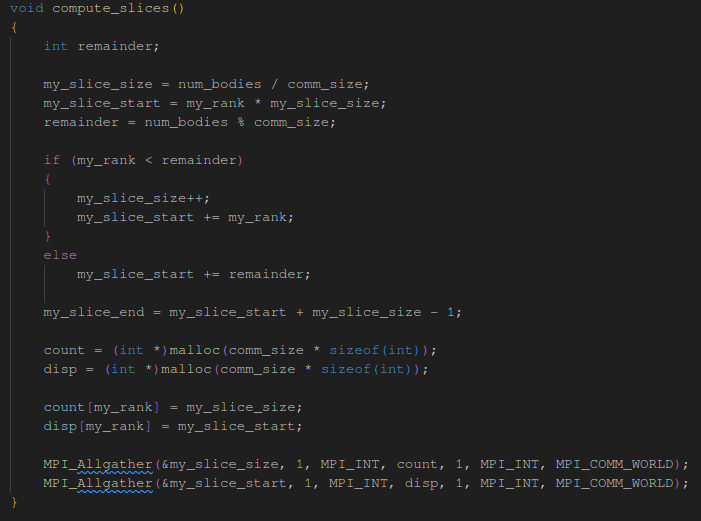
\includegraphics[width=\textwidth]{images/mpi_exh_1_1.png}
        \caption{Screenshot del frammento di codice di interesse di \texttt{mpi\_exh\_1.c}}
        \label{fig:mpi_exh_1_1}
    \end{figure}

    Inoltre, per poter effettuare le comunicazioni, è necessario che ogni processo crei a priori i datatype \texttt{MPI\_Vec3D} e \texttt{MPI\_Body} del tutto equivalenti ai due struct utilizzati nella versione seriale, ma in grado di essere trattati dalle comunicazioni di MPI. 

    \begin{figure}[H]
        \centering
        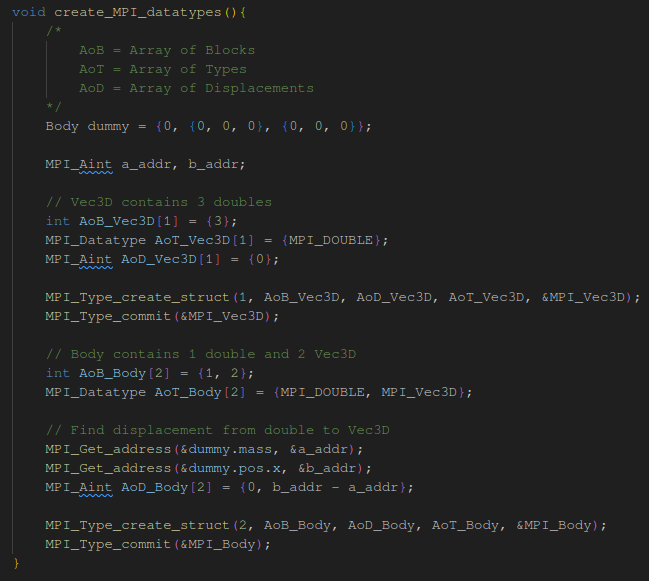
\includegraphics[width=\textwidth]{images/mpi_exh_1_2.png}
        \caption{Screenshot del frammento di codice di interesse di \texttt{mpi\_exh\_1.c}}
        \label{fig:mpi_exh_1_2}
    \end{figure}

    Una volta calcolata la suddivisione, i \textit{cicli for} vengono modificati per far sì che i processi svolgano solo i calcoli inerenti alla propria porzione di corpi. In fine solo il master process (rank = 0) scrive i risultati sull'output.

    Tuttavia, poiché la suddivisione dei corpi tra i processi potrebbe essere \textbf{non equa}, non è possibile utilizzare la funzione \texttt{MPI\_Allgheter}, rendendo necessario l'uso della funzione \texttt{MPI\_Allgheterv}, la quale condivide oltre alle informazioni sul tipo di dato trasmesso e ricevuto anche le informazioni sul \textbf{numero di blocchi} e il relativo \textbf{displacement} sull'array di destinazione. In tal modo, non è necessario aggiungere del padding ai dati inviati per riempire eventuali \textit{"buchi"}.

    \begin{figure}[H]
        \centering
        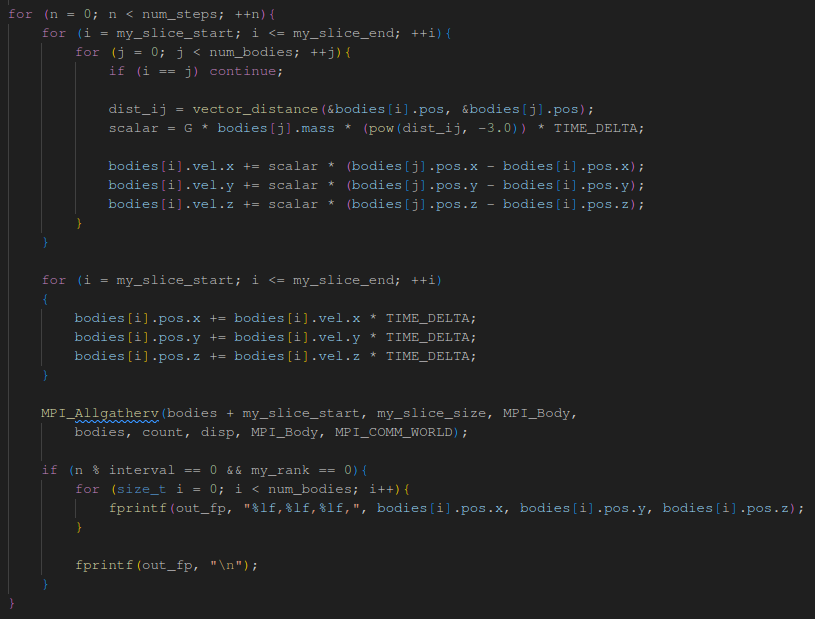
\includegraphics[width=\textwidth]{images/mpi_exh_1_3.png}
        \caption{Screenshot del frammento di codice di interesse di \texttt{mpi\_exh\_1.c}}
        \label{fig:mpi_exh_1_3}
    \end{figure}

    A seguito dell'analisi precedente, dunque, possiamo stabilire che, per natura stessa dell'algoritmo, l'uso di una parallelizzazione a memoria distribuita risulta \textbf{inefficiente} rispetto a quella a memoria condivisa. Tale risultato si evince dall'elevata mole di comunicazioni richieste tra i vari processi (una per passo della simulazione), rallentando significativamente il programma. In particolare, all'aumentare dei processi involti nella parallelizzazione, tali comunicazioni richiedono un \textbf{vasto overhead}.

    \begin{figure}[H]
        \centering
        
        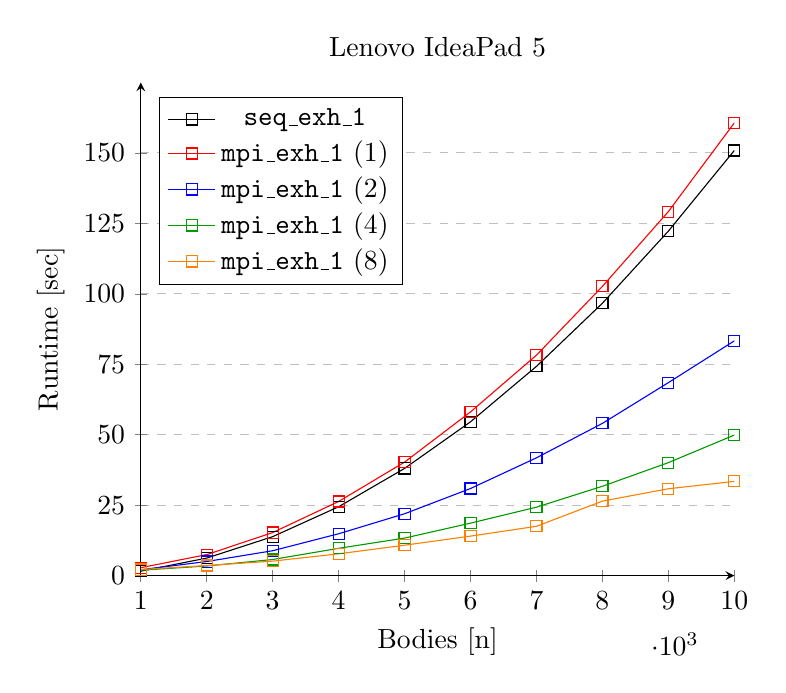
\begin{tikzpicture}
            \begin{axis}[
                axis lines = center,
                hide obscured x ticks=false,
                hide obscured y ticks=false,
                xlabel={Bodies [n]},
                ylabel={Runtime [sec]},
                ylabel near ticks,
                xlabel near ticks,
                xmin=1000, xmax=10000,
                ymin=0, ymax=175,
                xtick={1000, 2000, 3000, 4000, 5000, 6000, 7000, 8000, 9000, 10000},
                ytick={0, 25, 50, 75, 100, 125, 150},
                legend pos=north west,
                ymajorgrids=true,
                grid style=dashed,
                scaled x ticks= base 10:-3,
                scale=1.1,
                title=Lenovo IdeaPad 5
            ]
            
            \addplot[
                color=black,
                mark=square,
                ]
                coordinates {
                (1000, 1.588418460)
                (2000, 6.230024672)
                (3000, 13.835473919)
                (4000, 24.445233798)
                (5000, 38.049215651)
                (6000, 54.591586947)
                (7000, 74.272990847)
                (8000, 96.675407171)
                (9000, 122.254725814)
                (10000, 150.870804667)
                };

            \addplot[
                color=red,
                mark=square,
                ]
                coordinates {
                (1000, 2.82194710)
                (2000, 7.46232080)
                (3000, 15.28543472)
                (4000, 26.31298161)
                (5000, 40.28574896)
                (6000, 58.09200668)
                (7000, 78.24205589)
                (8000, 102.65228033)
                (9000, 129.18786526)
                (10000, 160.66591072)
                };
            
            \addplot[
                color=blue,
                mark=square,
                ]
                coordinates {
                (1000, 2.10146713)
                (2000, 5.00848913)
                (3000, 8.84116411)
                (4000, 14.86012936)
                (5000, 21.95946169)
                (6000, 30.91917086)
                (7000, 41.80733633)
                (8000, 54.03394318)
                (9000, 68.48802280)
                (10000, 83.31656694)
                };

            \addplot[
                color=green!60!black,
                mark=square,
                ]
                coordinates {
                (1000, 1.92610025)
                (2000, 3.41965580)
                (3000, 5.72816467)
                (4000, 9.69374704)
                (5000, 13.32703781)
                (6000, 18.63166380)
                (7000, 24.29812860)
                (8000, 31.71978426)
                (9000, 40.10225010)
                (10000, 49.89095783)
                };

            
            \addplot[
                color=orange,
                mark=square,
                ]
                coordinates {
                (1000, 2.16701412)
                (2000, 3.59521055)
                (3000, 5.15208197)
                (4000, 7.74772739)
                (5000, 10.79919720)
                (6000, 14.02549171)
                (7000, 17.50465584)
                (8000, 26.44839287)
                (9000, 30.83210230)
                (10000, 33.45039320)
                };
    

            \legend{\texttt{seq\_exh\_1},\texttt{mpi\_exh\_1} (1), \texttt{mpi\_exh\_1} (2), \texttt{mpi\_exh\_1} (4), \texttt{mpi\_exh\_1} (8), }
            \end{axis}
        \end{tikzpicture}

        \quad 
        
        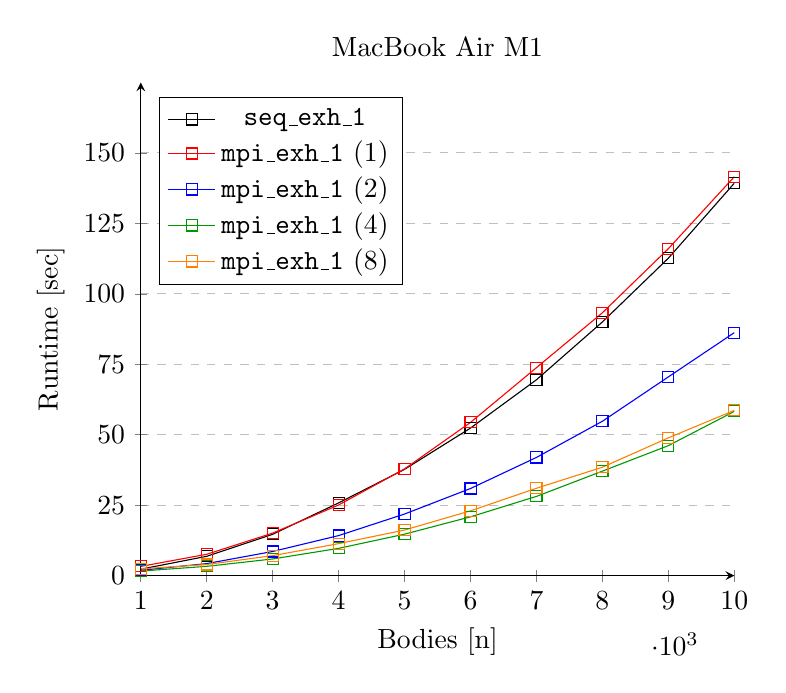
\begin{tikzpicture}
            \begin{axis}[
                axis lines = center,
                hide obscured x ticks=false,
                hide obscured y ticks=false,
                xlabel={Bodies [n]},
                ylabel={Runtime [sec]},
                ylabel near ticks,
                xlabel near ticks,
                xmin=1000, xmax=10000,
                ymin=0, ymax=175,
                xtick={1000, 2000, 3000, 4000, 5000, 6000, 7000, 8000, 9000, 10000},
                ytick={0, 25, 50, 75, 100, 125, 150},
                legend pos=north west,
                ymajorgrids=true,
                grid style=dashed,
                scaled x ticks= base 10:-3,
                scale=1.1,
                title=MacBook Air M1
            ]
            
            \addplot[
                color=black,
                mark=square,
                ]
                coordinates {
                (1000, 2.29056454)
                (2000, 6.86578417)
                (3000, 14.67731190)
                (4000, 25.80976057)
                (5000, 37.72510433)
                (6000, 52.36848545)
                (7000, 69.51298285)
                (8000, 90.02810717)
                (9000, 112.65391874)
                (10000, 139.26667118)
                };

            \addplot[
                color=red,
                mark=square,
                ]
                coordinates {
                (1000, 3.27747202)
                (2000, 7.58044624)
                (3000, 15.09387636)
                (4000, 25.06907368)
                (5000, 37.87850428)
                (6000, 54.37706757)
                (7000, 73.81191254)
                (8000, 93.28557825)
                (9000, 116.03542852)
                (10000, 141.55162001)
                };
            
            \addplot[
                color=blue,
                mark=square,
                ]
                coordinates {
                (1000, 1.89387608)
                (2000, 4.27036190)
                (3000, 8.57425261)
                (4000, 14.21473742)
                (5000, 21.86949396)
                (6000, 30.92402267)
                (7000, 41.95113945)
                (8000, 54.79537010)
                (9000, 70.52728844)
                (10000, 86.23026466)
                };

            \addplot[
                color=green!60!black,
                mark=square,
                ]
                coordinates {
                (1000, 1.63046074)
                (2000, 3.29796934)
                (3000, 5.91780043)
                (4000, 9.68749619)
                (5000, 14.72253084)
                (6000, 20.87375116)
                (7000, 28.12389851)
                (8000, 37.08254623)
                (9000, 46.13995695)
                (10000, 58.28085327)
                };
            
            \addplot[
                color=orange,
                mark=square,
                ]
                coordinates {
                (1000, 2.40023661)
                (2000, 3.95483971)
                (3000, 7.10325432)
                (4000, 11.35675001)
                (5000, 16.18534422)
                (6000, 23.00083303)
                (7000, 31.00731754)
                (8000, 38.47862291)
                (9000, 48.89983892)
                (10000, 58.65127182)
                };
    

            \legend{\texttt{seq\_exh\_1},\texttt{mpi\_exh\_1} (1), \texttt{mpi\_exh\_1} (2), \texttt{mpi\_exh\_1} (4), \texttt{mpi\_exh\_1} (8), }
            \end{axis}
        \end{tikzpicture}

        \caption{Confronto delle performance di \texttt{seq\_exh\_1} e \texttt{mpi\_exh\_1} su 100 passi di simulazione da 1000 a 10000 corpi. I numeri tra parentesi nella legenda del grafico indicano il numero di thread attivi}
        \label{fig:mpi_exh_graph}
    \end{figure}

    \newpage

    \subsection{Riduzione e localizzazione dei dati trasmessi}

    Poiché le comunicazioni comunicazioni risultano essere il \textit{bottleneck} della versione \texttt{mpi\_exh\_1}, risulta ovvio analizzare \textbf{modalità per alleggerire} tali comunicazioni riducendo la quantità dei dati trasmessi da esse.
    
    In particolare, notiamo che al fine di poter eseguire il passo successivo della simulazione, è sufficiente che ogni processo trasmetta a tutti gli altri processi solo ed esclusivamente le proprie \textbf{nuove posizioni} in quanto le masse dei corpi rimangono invariate durante la simulazione e in quanto le nuove velocità dei corpi esterni alla porzione assegnata al processo stesso non siano rilevanti per il calcolo. Di conseguenza, i dati comunicati da ogni processo si riducono $\frac{n}{p} \cdot 7$ double a solo $\frac{n}{p} \cdot 3$ double.

    \begin{figure}[H]
        \centering
        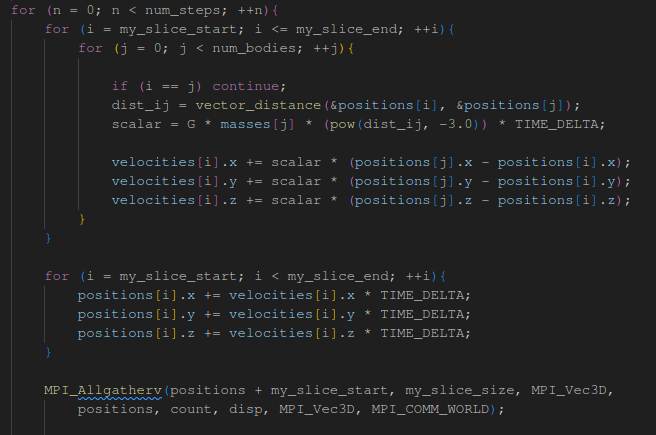
\includegraphics[width=\textwidth]{images/mpi_exh_2.png}
        \caption{Screenshot del frammento di codice di interesse di \texttt{mpi\_exh\_2.c}}
        \label{fig:mpi_exh_2}
    \end{figure}
    
    Tuttavia, i test effettuati dimostrano che riducendo la dimensione del pacchetto trasmesso da ogni processo i tempi di comunicazione rimangono \textbf{per lo più invariati}, rendendo tale cambiamento utile solo superficialmente.

    \begin{figure}[H]
        \centering
        
        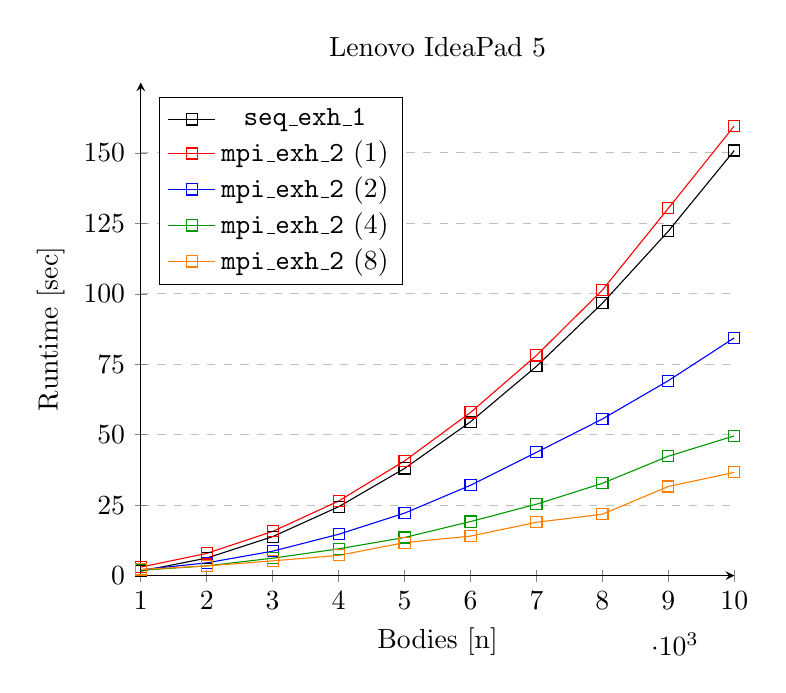
\begin{tikzpicture}
            \begin{axis}[
                axis lines = center,
                hide obscured x ticks=false,
                hide obscured y ticks=false,
                xlabel={Bodies [n]},
                ylabel={Runtime [sec]},
                ylabel near ticks,
                xlabel near ticks,
                xmin=1000, xmax=10000,
                ymin=0, ymax=175,
                xtick={1000, 2000, 3000, 4000, 5000, 6000, 7000, 8000, 9000, 10000},
                ytick={0, 25, 50, 75, 100, 125, 150},
                legend pos=north west,
                ymajorgrids=true,
                grid style=dashed,
                scaled x ticks= base 10:-3,
                scale=1.1,
                title=Lenovo IdeaPad 5
            ]
            
            \addplot[
                color=black,
                mark=square,
                ]
                coordinates {
                (1000, 1.588418460)
                (2000, 6.230024672)
                (3000, 13.835473919)
                (4000, 24.445233798)
                (5000, 38.049215651)
                (6000, 54.591586947)
                (7000, 74.272990847)
                (8000, 96.675407171)
                (9000, 122.254725814)
                (10000, 150.870804667)
                };

            \addplot[
                color=red,
                mark=square,
                ]
                coordinates {
                (1000, 3.04153013)
                (2000, 7.88631296)
                (3000, 15.70073795)
                (4000, 26.46183491)
                (5000, 40.72397614)
                (6000, 57.90560961)
                (7000, 78.14709234)
                (8000, 101.35953903)
                (9000, 130.36002970)
                (10000, 159.60092449)
                };
            
            \addplot[
                color=blue,
                mark=square,
                ]
                coordinates {
                (1000, 2.09063673)
                (2000, 4.53376913)
                (3000, 8.68055868)
                (4000, 14.67308044)
                (5000, 22.19207096)
                (6000, 32.05901337)
                (7000, 43.74659681)
                (8000, 55.59438610)
                (9000, 69.19136429)
                (10000, 84.38146210)
                };

            \addplot[
                color=green!60!black,
                mark=square,
                ]
                coordinates {
                (1000, 1.90050316)
                (2000, 3.46576357)
                (3000, 6.20071745)
                (4000, 9.50769281)
                (5000, 13.53752708)
                (6000, 19.20171881)
                (7000, 25.35158873)
                (8000, 32.76420259)
                (9000, 42.38885784)
                (10000, 49.61076498)
                };

            
            \addplot[
                color=orange,
                mark=square,
                ]
                coordinates {
                (1000, 2.19370508)
                (2000, 3.44379902)
                (3000, 5.24651003)
                (4000, 7.18327522)
                (5000, 11.72652006)
                (6000, 14.03149843)
                (7000, 18.93168402)
                (8000, 21.80226278)
                (9000, 31.6392088)
                (10000, 36.63834620)
                };
    

            \legend{\texttt{seq\_exh\_1},\texttt{mpi\_exh\_2} (1), \texttt{mpi\_exh\_2} (2), \texttt{mpi\_exh\_2} (4), \texttt{mpi\_exh\_2} (8), }
            \end{axis}
        \end{tikzpicture}

        \quad 
        
        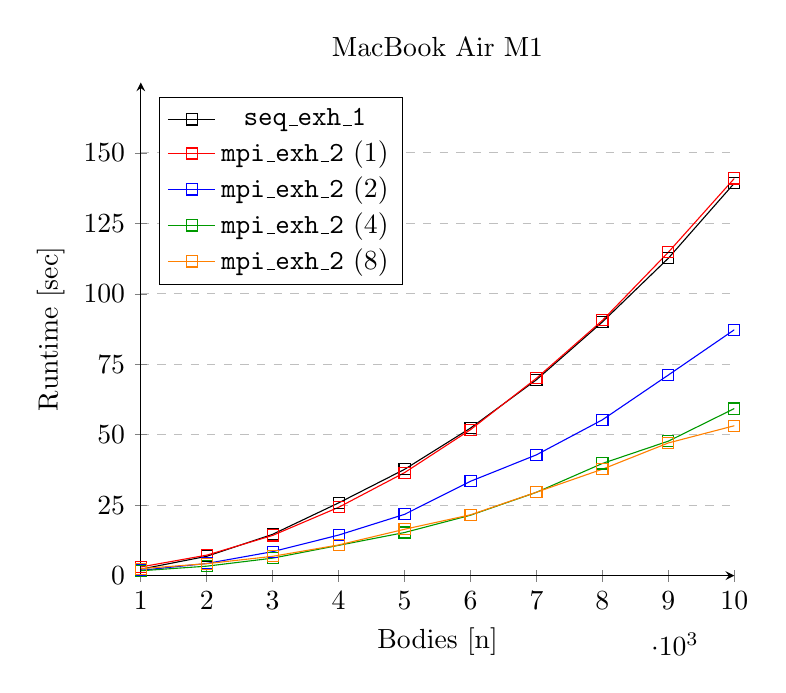
\begin{tikzpicture}
            \begin{axis}[
                axis lines = center,
                hide obscured x ticks=false,
                hide obscured y ticks=false,
                xlabel={Bodies [n]},
                ylabel={Runtime [sec]},
                ylabel near ticks,
                xlabel near ticks,
                xmin=1000, xmax=10000,
                ymin=0, ymax=175,
                xtick={1000, 2000, 3000, 4000, 5000, 6000, 7000, 8000, 9000, 10000},
                ytick={0, 25, 50, 75, 100, 125, 150},
                legend pos=north west,
                ymajorgrids=true,
                grid style=dashed,
                scaled x ticks= base 10:-3,
                scale=1.1,
                title=MacBook Air M1
            ]
            
            \addplot[
                color=black,
                mark=square,
                ]
                coordinates {
                (1000, 2.29056454)
                (2000, 6.86578417)
                (3000, 14.67731190)
                (4000, 25.80976057)
                (5000, 37.72510433)
                (6000, 52.36848545)
                (7000, 69.51298285)
                (8000, 90.02810717)
                (9000, 112.65391874)
                (10000, 139.26667118)
                };

            \addplot[
                color=red,
                mark=square,
                ]
                coordinates {
                (1000, 3.07966280)
                (2000, 7.27002716)
                (3000, 14.27405405)
                (4000, 24.24649668)
                (5000, 36.55378771)
                (6000, 51.80325127)
                (7000, 70.05103159)
                (8000, 90.57968378)
                (9000, 114.77531433)
                (10000, 140.94219446)
                };
            
            \addplot[
                color=blue,
                mark=square,
                ]
                coordinates {
                (1000, 1.87613726)
                (2000, 4.31389713)
                (3000, 8.51528978)
                (4000, 14.39540386)
                (5000, 21.75190258)
                (6000, 33.48335600)
                (7000, 42.87297535)
                (8000, 55.30720901)
                (9000, 71.19776869)
                (10000, 87.25897789)
                };

            \addplot[
                color=green!60!black,
                mark=square,
                ]
                coordinates {
                (1000, 1.73021221)
                (2000, 3.35996389)
                (3000, 6.20994139)
                (4000, 10.74384642)
                (5000, 15.30670547)
                (6000, 21.44735622)
                (7000, 29.57401180)
                (8000, 39.81125402)
                (9000, 47.73064184)
                (10000, 59.29170227)
                };
            
            \addplot[
                color=orange,
                mark=square,
                ]
                coordinates {
                (1000, 2.48461819)
                (2000, 4.24743700)
                (3000, 6.85591221)
                (4000, 10.89073896)
                (5000, 16.46069336)
                (6000, 21.58819008)
                (7000, 29.62332535)
                (8000, 37.78240061)
                (9000, 47.09512568)
                (10000, 53.19379139)
                };
    

            \legend{\texttt{seq\_exh\_1},\texttt{mpi\_exh\_2} (1), \texttt{mpi\_exh\_2} (2), \texttt{mpi\_exh\_2} (4), \texttt{mpi\_exh\_2} (8), }
            \end{axis}
        \end{tikzpicture}

        \caption{Confronto delle performance di \texttt{seq\_exh\_1} e \texttt{mpi\_exh\_2} su 100 passi di simulazione da 1000 a 10000 corpi. I numeri tra parentesi nella legenda del grafico indicano il numero di thread attivi}
        \label{fig:mpi_2_exh_graph}
    \end{figure}

    \newpage
    
    Nonostante ciò, è possibile ottenere un miglioramento delle prestazioni di circa il 15\% riscrivendo le velocità dei corpi utilizzati all'interno di un \textbf{array più piccolo} e lavorando su quest'ultimo anziché sul vettore che contiene le informazione di tutti i corpi. 

    \begin{figure}[H]
        \centering
        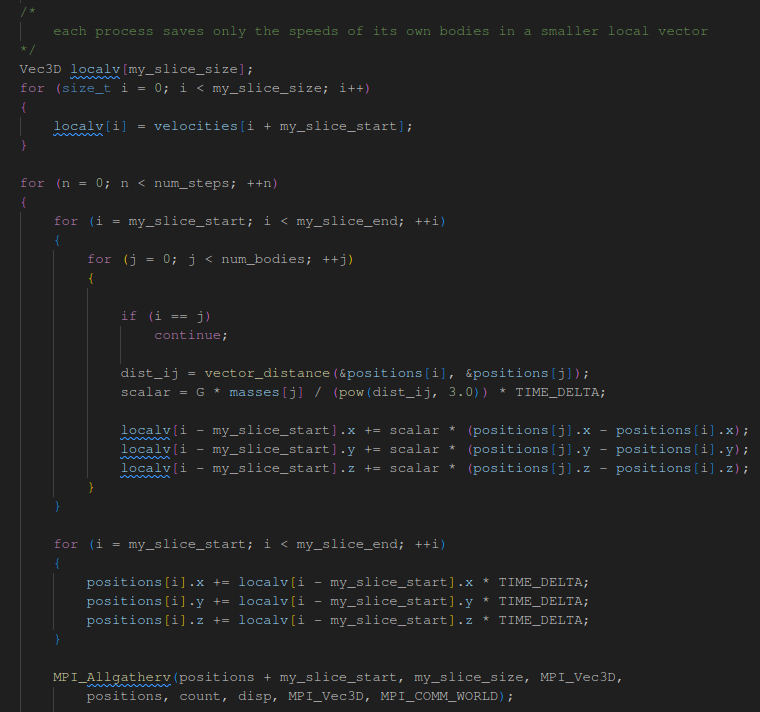
\includegraphics[width=\textwidth]{images/mpi_exh_3.png}
        \caption{Screenshot del frammento di codice di interesse di \texttt{mpi\_exh\_3.c}}
        \label{fig:mpi_exh_3}
    \end{figure}

    \begin{figure}[H]
        \centering
        
        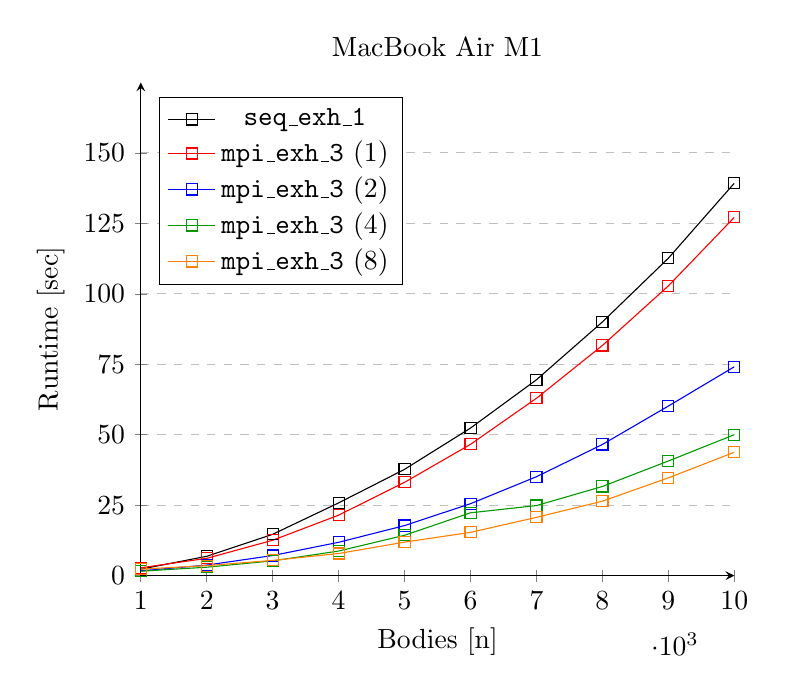
\begin{tikzpicture}
            \begin{axis}[
                axis lines = center,
                hide obscured x ticks=false,
                hide obscured y ticks=false,
                xlabel={Bodies [n]},
                ylabel={Runtime [sec]},
                ylabel near ticks,
                xlabel near ticks,
                xmin=1000, xmax=10000,
                ymin=0, ymax=175,
                xtick={1000, 2000, 3000, 4000, 5000, 6000, 7000, 8000, 9000, 10000},
                ytick={0, 25, 50, 75, 100, 125, 150},
                legend pos=north west,
                ymajorgrids=true,
                grid style=dashed,
                scaled x ticks= base 10:-3,
                scale=1.1,
                title=MacBook Air M1
            ]
            
            \addplot[
                color=black,
                mark=square,
                ]
                coordinates {
                (1000, 2.29056454)
                (2000, 6.86578417)
                (3000, 14.67731190)
                (4000, 25.80976057)
                (5000, 37.72510433)
                (6000, 52.36848545)
                (7000, 69.51298285)
                (8000, 90.02810717)
                (9000, 112.65391874)
                (10000, 139.26667118)
                };

            \addplot[
                color=red,
                mark=square,
                ]
                coordinates {
                (1000, 2.78916407)
                (2000, 6.13773680)
                (3000, 12.55515623)
                (4000, 21.46174383)
                (5000, 33.11679363)
                (6000, 46.59499741)
                (7000, 62.94386387)
                (8000, 81.68642998)
                (9000, 102.83041430)
                (10000, 127.15266371)
                };
            
            \addplot[
                color=blue,
                mark=square,
                ]
                coordinates {
                (1000, 1.70515919)
                (2000, 3.74255753)
                (3000, 7.14080381)
                (4000, 11.83334875)
                (5000, 17.76290512)
                (6000, 25.53192616)
                (7000, 35.10490131)
                (8000, 46.55611229)
                (9000, 60.18213367)
                (10000, 74.12223911)
                };

            \addplot[
                color=green!60!black,
                mark=square,
                ]
                coordinates {
                (1000, 1.56900501)
                (2000, 2.99602413)
                (3000, 5.24200821)
                (4000, 8.73013878)
                (5000, 14.32354593)
                (6000, 22.30249739)
                (7000, 24.86654472)
                (8000, 31.64473295)
                (9000, 40.67955875)
                (10000, 50.02179480)
                };
            
            \addplot[
                color=orange,
                mark=square,
                ]
                coordinates {
                (1000, 2.30836582)
                (2000, 3.553792477)
                (3000, 5.405865669)
                (4000, 7.854512215)
                (5000, 11.890188694)
                (6000, 15.357589245)
                (7000, 20.680476189)
                (8000, 26.427812099)
                (9000, 34.701496124)
                (10000, 43.783582211)
                };

            \legend{\texttt{seq\_exh\_1},\texttt{mpi\_exh\_3} (1), \texttt{mpi\_exh\_3} (2), \texttt{mpi\_exh\_3} (4), \texttt{mpi\_exh\_3} (8), }
            \end{axis}
        \end{tikzpicture}

        \caption{Confronto delle performance di \texttt{seq\_exh\_1} e \texttt{mpi\_exh\_3} su 100 passi di simulazione da 1000 a 10000 corpi. I numeri tra parentesi nella legenda del grafico indicano il numero di thread attivi}
        \label{fig:mpi_3_exh_graph}
    \end{figure}

    Tuttavia, tale miglioramento viene ottenuto \underline{solo ed esclusivamente} sul dispositivo MacBook Air M1, mentre per il dispositivo Lenovo IdeaPad 5 i risultati rimangono ancora una volta \textbf{invariati}.

    \newpage

    \section{Analisi dello speed-up e dell'efficienza}

    Tramite i dati inerenti al runtime delle varie versioni parallelizzate e non mostrati nelle sezioni precedenti, consideriamo lo \textbf{speed-up} e l'\textbf{efficienza} ottenute da ognuna di tali versioni rispetto all'implementazione sequenziale \texttt{seq\_exh\_1} nel caso con 10000 corpi.

    In particolare, per entrambi i dispositivi e per ogni modalità di implementazione parallela viene riportato il programma i cui runtime medi hanno performato tendenzialmente meglio, ossia i programmi \texttt{omp\_exh\_3} e \texttt{mpi\_exh\_3}.

    \begin{figure}[H]
        \centering

        \begin{tabular}{ l | c | c | c }
            \textbf{Programma} & \textbf{Runtime} & \textbf{Speed-up} & \textbf{Efficienza}\\
            \hline
            \texttt{seq\_exh\_1} & 150.870804667 & 1.000000000 & 1.00 \\
            \hline
            \texttt{omp\_exh\_3 (1)} & 166.075013638 & 0.908449750 & 0.90 \\
            \texttt{omp\_exh\_3 (2)} & 92.657269955 & 1.628267320 & 0.81 \\
            \texttt{omp\_exh\_3 (4)} & 50.705098152 & 2.975456318 & 0.74 \\
            \texttt{omp\_exh\_3 (8)} & 31.612117290 & 4.772562473 & 0.59 \\
            \hline
            \texttt{mpi\_exh\_3 (1)} & 159.60092449 & 0.945300318 & 0.94 \\
            \texttt{mpi\_exh\_3 (2)} & 84.38146210 & 1.787961490 & 0.89 \\
            \texttt{mpi\_exh\_3 (4)} & 49.61076498 & 3.041090068 & 0.76 \\
            \texttt{mpi\_exh\_3 (8)} & 36.63834620 & 4.117838830 & 0.51 \\
        \end{tabular}
        \caption{Statistiche per dispositivo Lenovo IdeaPad 5}
        \label{fig:stats_ip5_1}
    \end{figure}

    \begin{figure}[H]
        \centering

        \begin{tabular}{ l | c | c | c }
            \textbf{Programma} & \textbf{Runtime} & \textbf{Speed-up} & \textbf{Efficienza}\\
            \hline
            \texttt{seq\_exh\_1} & 139.26667118 & 1.000000000 & 1.00 \\
            \hline
            \texttt{omp\_exh\_3 (1)} & 142.753837109 & 0.975572174 & 0.97 \\
            \texttt{omp\_exh\_3 (2)} & 101.364573956 & 1.373918577 & 0.68 \\
            \texttt{omp\_exh\_3 (4)} & 56.463528633 & 2.466488981 & 0.61 \\
            \texttt{omp\_exh\_3 (8)} & 51.738933086 & 2.691719038 & 0.33 \\
            \hline
            \texttt{mpi\_exh\_3 (1)} & 127.15266371 & 1.095271362 & 1.09 \\
            \texttt{mpi\_exh\_3 (2)} & 74.12223911 & 1.878878362 & 0.93 \\
            \texttt{mpi\_exh\_3 (4)} & 50.02179480 & 2.784119837 & 0.69 \\
            \texttt{mpi\_exh\_3 (8)} & 43.783582211 & 3.180796640 & 0.39 \\
        \end{tabular}
        \caption{Statistiche per dispositivo MacBook Air M1}
        \label{fig:stats_m1_1}
    \end{figure}

    \addtocontents{toc}{\protect\newpage}

    \chapter{Simulazione tramite algoritmo di Barnes-Hut}

    \section{Descrizione dell'algoritmo}

    L'\textbf{algoritmo di Barnes-Hut} è uno dei metodi di approssimazione più utilizzato per problema degli $n$ corpi. I punti nello spazio vengono considerati come un \textbf{piano cartesiano tridimensionale} i cui assi $x,y$ e $z$ rappresentano rispettivamente la larghezza (Ovest-Est), l'altezza (Sopra-Sotto) e la profondità (Nord-Sud) dei corpi
        
    \begin{figure}[H]
        \centering
        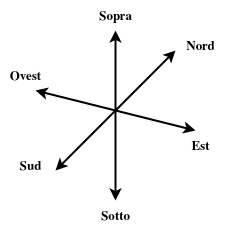
\includegraphics[scale=0.7]{images/plane.png}
        \caption{Suddivisione dello spazio nelle otto direzioni spaziali}
        \label{fig:plane}
    \end{figure}

    Lo \textbf{spazio occupato dai corpi} viene considerato come un cubo $\ell \times \ell \times \ell$, dove $\ell$ è il doppio della distanza massima tra l'origine dello spazio (ossia il punto $(0,0,0)$) e gli $n$ corpi.

    Tale cubo viene \textbf{suddiviso in $8$ sotto-cubi} di dimensione $\frac{\ell}{2} \times \frac{\ell}{2} \times \frac{\ell}{2}$. Tali cubi vengono indicati come una combinazione di \textbf{tre direzioni spaziali}:
    \begin{itemize}
        \item \textbf{Upper} e \textbf{Lower}, ossia tutti i cubi situati rispettivamente nella bisezione \textit{superiore} e \textit{inferiore} della coordinata $y$
        \item \textbf{North} e \textbf{South}, ossia tutti i cubi situati rispettivamente nella bisezione \textit{frontale} e \textit{posteriore} della coordinata $z$
        \item \textbf{West} e \textbf{East}, ossia tutti i cubi situati rispettivamente nella bisezione \textit{sinistra} e \textit{destra} della coordinata $x$
    \end{itemize}

    In totale, dunque, i sotto-cubi sono identificati dai seguenti acronimi:
    \texttt{UNW}, \texttt{UNE}, \texttt{USW}, \texttt{USE}, \texttt{LNW}, \texttt{LNE}, \texttt{LSW}, \texttt{LSE}

    Successivamente, se uno dei sotto-cubi contiene al suo interno più di un corpo, tale sotto-cubo viene \textbf{sezionato nuovamente}, ripetendo l'intero processo ricorsivamente finché ogni sotto-cubo non contiene un solo corpo.

    \begin{figure}[H]
        \centering
        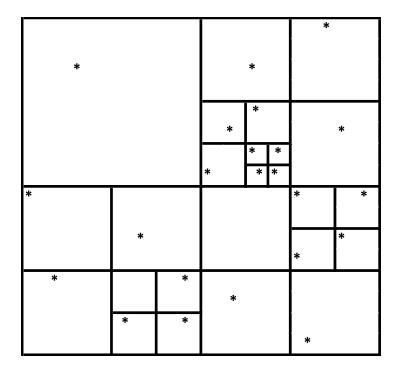
\includegraphics[scale=0.7]{images/4tree.png}
        \caption{Esempio bidimensionale della suddivisione}
        \label{fig:4tree}
    \end{figure}

    Una volta suddiviso lo spazio, l'algoritmo procede calcolando gli \textbf{\textit{"pseudo-corpi"}} di ogni sotto-cubo: se all'interno di un sotto-cubo vi sono $k$ corpi, la posizione e la massa dello pseudo-corpo associato a tale sotto-cubo corrisponderanno rispettivamente al centro della massa e alla massa totale ricavate tramite i $k$ corpi.

    Ad esempio, se un sotto-cubo contiene i corpi $b_1, \ldots, b_4$, il centro della massa del suo pseudo-corpo corrisponderà a:
    \[\vec{c} = \frac{m_1\vec{p_1} + \ldots + m_4 \vec{p_4}}{m_1 + \ldots + m_4}\]

    In particolare, notiamo che se un sotto-cubo contiene un solo corpo, allora il suo pseudo-corpo \textbf{coincide} con tale unico corpo.

    Una volta calcolati tutti gli pseudo-corpi, l'algoritmo procede calcolando le interazioni tra ogni corpo. In particolare, tramite un valore $\theta$ dettato a priori, tali interazioni possono essere \textbf{approssimate} con l'interazione con uno pseudo-corpo:
    \begin{enumerate}
        \item Sia $b_i$ il corpo di cui attualmente si sta calcolando l'interazione
        \item Partendo dal cubo originale, l'algoritmo calcola il rapporto $\frac{s}{d}$, dove $s$ è il \textbf{lato} del cubo e $d$ e la \textbf{distanza vettoriale} tra $b_i$ e lo pseudo-corpo $w$ associato a tale cubo
        \item Se $\frac{s}{d} < \theta$, allora l'algoritmo approssimerà l'interazione tra $b_i$ e tutti i corpi contenuti nel cubo calcolando direttamente l'interazione tra $b_i$ e $w$. Altrimenti, l'algoritmo procederà ricorsivamente nei sotto-cubi. 
    \end{enumerate}
    
    Tali approssimazioni permettono di \textbf{risparmiare} una grande mole di calcoli, riducendo l'andamento asintotico del programma a $O(n \log n)$. È opportuno notare,inoltre, che il valore scelto per $\theta$ risulti fondamentale:
    \begin{itemize}
        \item Se $\theta = 0.0$, l'algoritmo non approssimerà mai il calcolo, facendo degenerare l'intero algoritmo in una versione più complessa e lenta dell'im-plementazione esaustiva della simulazione
        \item Se $\theta = 1.0$, le prestazioni dell'algoritmo risultano estremamente migliori rispetto all'implementazione esaustiva, producendo tuttavia un'errore di approssimazione rilevante, ma tuttavia abbastanza trascurabile
        \item Se $\theta \geq 1.25$, l'errore generato dall'approssimazione risulta eccessivamente alto
    \end{itemize}

    In particolare, è necessario notare che, indipendentemente dal valore $\theta$ scelto, l'errore risulta essere \textbf{inversamente proporzionale} al numero $n$ di corpi involti nella simulazione.

    Dopo un'attenta analisi, è stato scelto di utilizzare il \textbf{valore $\mathbf{\theta = 0.5}$}, in quanto l'incremento delle performance risulti non molto distante da quello ottenuto con il valore $\theta = 1.0$, presentando tuttavia un'errore pari a $0.0001\%$ nella maggior parte delle simulazioni effettuate.
    
    \quad

    \section{Implementazione sequenziale}

    \subsection{Struttura dati e funzioni principali}

    Tramite la descrizione della sezione precedente, l'implementazione sequenziale dell'algoritmo viene interamente ridotta all'implementazione di una \textbf{struttura dati} che possa permettere di svolgere le varie operazioni efficientemente.
    
    In particolare, per rappresentare la suddivisione ricorsiva dello spazio occupato dai corpi, risulta intuitivo l'uso di un \textbf{oct-tree}, ossia un albero i cui nodi possono possedere fino ad \textit{8 figli}. Tali figli vengono memorizzati tramite un array di 8 puntatori ad altri nodi, dove ogni indice rappresenta uno specifico figlio:
    \begin{center}
        \begin{tabular}{c | c | c | c | c | c | c | c}
            \textbf{0} & \textbf{1} & \textbf{2} & \textbf{3} & \textbf{4} & \textbf{5} & \textbf{6} & \textbf{7}\\
            \hline
            \texttt{UNW} & \texttt{UNE} & \texttt{USW} & \texttt{USE} & \texttt{LNW} & \texttt{LNE} & \texttt{LSW} & \texttt{LSE}
        \end{tabular}
    \end{center}

    Oltre ai puntatori ai figli, ogni nodo dovrà memorizzare anche informazioni inerenti ai \textbf{confini} dello spazio rappresentato dal sotto-cubo (\textit{bounding box}), informazioni inerenti al proprio \textbf{pseudo-corpo} associato e informazioni inerenti all'attuale \textbf{modalità}, la quale descrive lo stato attuale del sotto-cubo da esso rappresentato, ossia: \textit{vuoto}, \textit{singolo corpo} o \textit{suddiviso}.

    \begin{figure}[H]
        \centering
        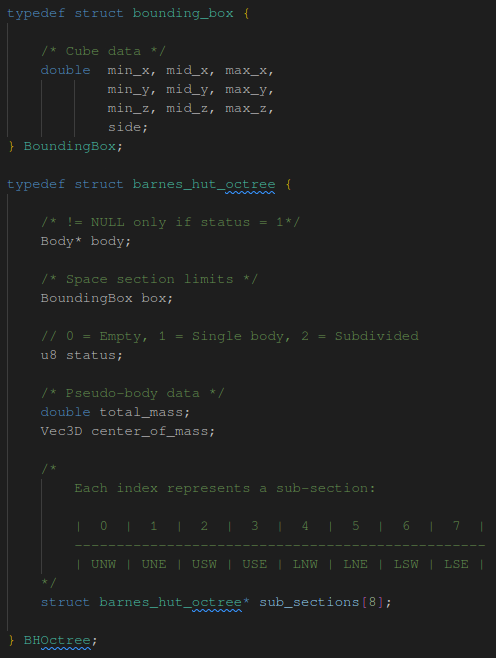
\includegraphics[width=0.75\textwidth]{images/bhoctree.png}
        \caption{Screenshot del frammento di codice di interesse di \texttt{bh\_octree\_1.h}}
        \label{fig:bhoctree_1}
    \end{figure}

    Per \textbf{generare} l'albero, è necessario calcolare quale sia la \textit{distanza massima} tra i corpi e il punto $(0,0,0)$, in modo da poter creare il primo nodo dell'albero corrispondente al cubo iniziale, per poi successivamente \textit{inserire} uno ad uno tutti i corpi ed infine calcolare gli \textit{pseudo-corpi}.

    \begin{figure}[H]
        \centering
        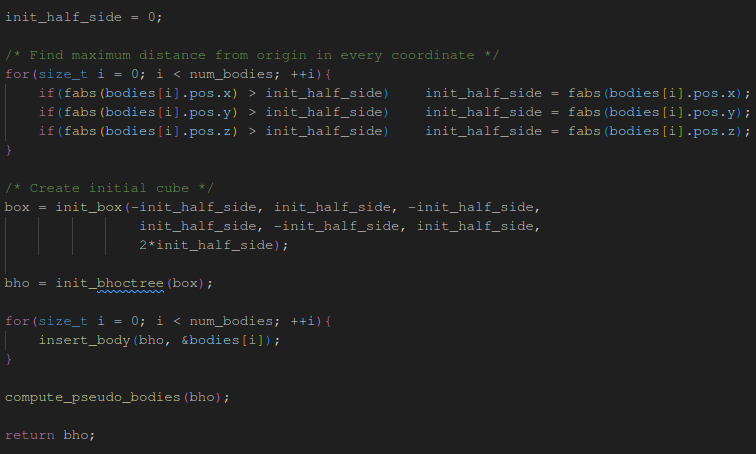
\includegraphics[width=\textwidth]{images/gen_bodies.png}
        \caption{Screenshot del frammento di codice della funzione \texttt{generate\_bodies\_bho()} presente in \texttt{bh\_octree\_1.c}}
        \label{fig:gen_bodies}
    \end{figure}

    Di fondamentale importanza risulta essere la procedura di \textbf{inserimento dei corpi}. Trattandosi della funzione principale per la costruzione dell'albero, è necessario che essa risulti essere il più efficiente possibile:
    \begin{itemize}
        \item Se il nodo in cui sta venendo inserito il corpo è nello stato \textbf{vuoto}, esso verrà impostato sullo stato \textit{singolo corpo}, conservando il puntatore al corpo inserito
        \item Se il nodo in cui sta venendo inserito il corpo è nello stato \textbf{singolo corpo}, esso verrà impostato sullo stato \textit{suddiviso}, per poi re-inserire in se stesso il corpo precedentemente conservato e il nuovo corpo
        \newpage
        \item Se il nodo in cui sta venendo inserito il corpo è nello stato \textbf{suddiviso}, verrà calcolata la sotto-sezione in cui inserire il corpo, ossia l'indice del figlio su cui propagare l'inserimento. Nel caso in cui il figlio non sia stato ancora creato, verrà calcolato il \textit{bounding box} corrispondente per poi creare suddetto figlio ed effettuare l'inserimento
    \end{itemize}

    \begin{figure}[H]
        \centering
        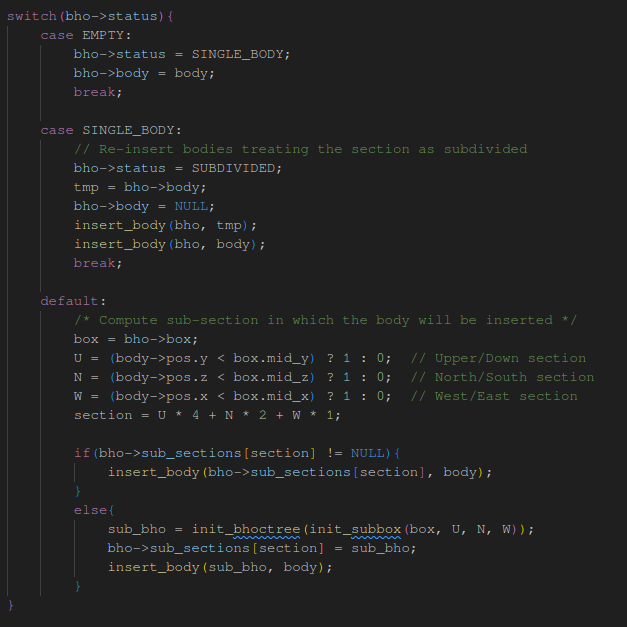
\includegraphics[width=\textwidth]{images/insert.png}
        \caption{Screenshot del frammento di codice della funzione \texttt{insert\_body()} presente in \texttt{bh\_octree\_1.c}}
        \label{fig:insert}
    \end{figure}
    
    \newpage

    Per quanto riguarda il \textbf{calcolo degli pseudo-corpi}, le proprietà algebriche delle formule mostrate nella sezione precedente permettono di ottimizzare notevolmente tale calcolo poiché lo pseudo-corpo di un nodo può essere calcolato tramite gli pseudo-corpi dei suoi figli, implicando che l'intero calcolo possa essere svolto tramite una \textbf{visita post-order}.

    \textbf{Esempio:}
    \begin{itemize}
        \item Supponiamo che la sezione $A$ contenga al suo interno le sezioni $B, C, D$
        \item Supponiamo inoltre che $A$ contenga i corpi $b_1, b_2, b_3, b_4$, che $B$ contenga i corpi $b_2, b_3$, che $C$ contenga il corpo $b_4$ e che $D$ contenga il corpo $b_1$ 
        \item Il centro della massa e la massa totale di $D$, ossia $\vec{c_D}$ e $m_D$, corrispondono a $\vec{p_1}$ e $m_1$ poiché $b_1$ risulta essere l'unico corpo al suo interno
        \item Il centro della massa e la massa totale di $C$, ossia $\vec{c_C}$ e $m_C$, corrispondono a $\vec{p_4}$ e $m_4$ poiché $b_4$ risulta essere l'unico corpo al suo interno
        \item Il centro della massa e la massa totale di $B$, ossia $\vec{c_B}$ e $m_B$, corrispondono a: 
        \[\vec{c_B} = \frac{m_2 \vec{p_2} + m_3 \vec{p_3}}{m_2 + m_3}\]

        \[m_B = m_2 + m_3\]

        \item Il centro della massa e la massa totale di $A$, ossia $\vec{c_A}$ e $m_B$, corrispondono a:
        \[\vec{c_A} = \frac{m_1 \vec{p_1} + m_2 \vec{p_2} + m_3 \vec{p_3} + m_4 \vec{p_4}}{m_1 + m_2 + m_3 + m_4}\]

        \[m_A = m_1 + m_2 + m_3 + m_4\]
        \item Notiamo quindi che:
        \[\vec{c_A} = \frac{m_1 \vec{p_1} + m_2 \vec{p_2} + m_3 \vec{p_3} + m_4 \vec{p_4}}{m_1 + m_2 + m_3 + m_4} = \frac{m_D \vec{c_D} + m_B \vec{c_B} + m_C \vec{c_C}}{m_D + m_B + m_C}\]

        \[m_A = m_1 + m_2 + m_3 + m_4 = m_D + m_B + m_C\]
    \end{itemize}

    \begin{figure}[H]
        \centering
        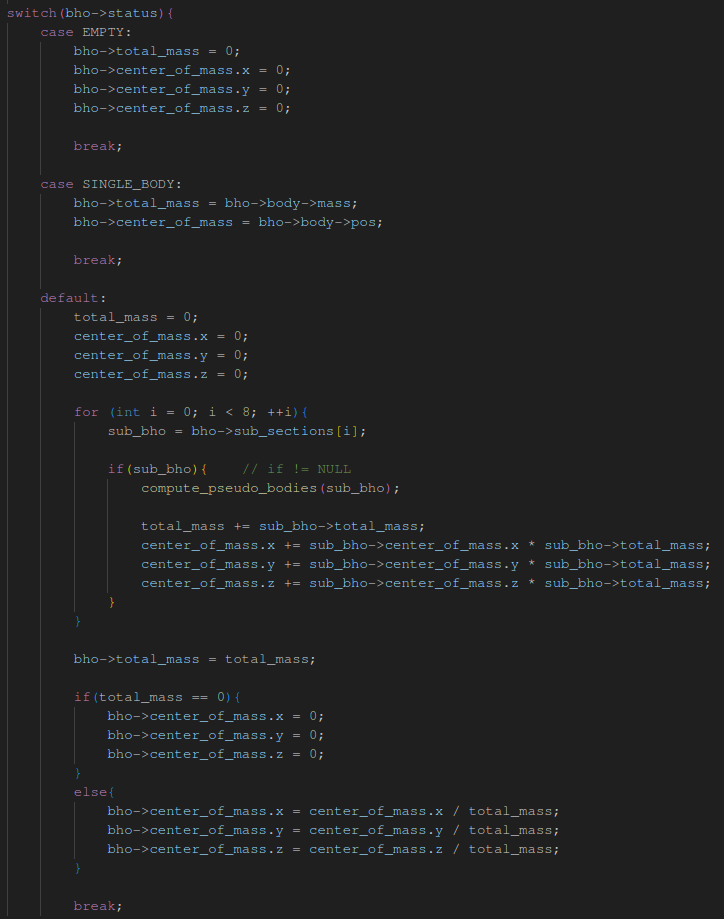
\includegraphics[width=\textwidth]{images/pseudo_bodies.png}
        \caption{Screenshot del frammento di codice della funzione \texttt{compute\_pseudo\_bodies()} presente in \texttt{bh\_octree\_1.c}}
        \label{fig:pseudo_bodies}
    \end{figure}

    Una volta costruito l'albero e calcolati gli pseudo-corpi, l'algoritmo procede con il calcolare l'\textbf{aggiornamento delle velocità}. Dato il corpo $b_i$ attualmente considerato, viene computato se approssimare il calcolo o no tramite il rateo di $\frac{s}{d}$ e il valore $\theta$ tramite una \textbf{visita post-order}.
    
    \begin{figure}[H]
        \centering
        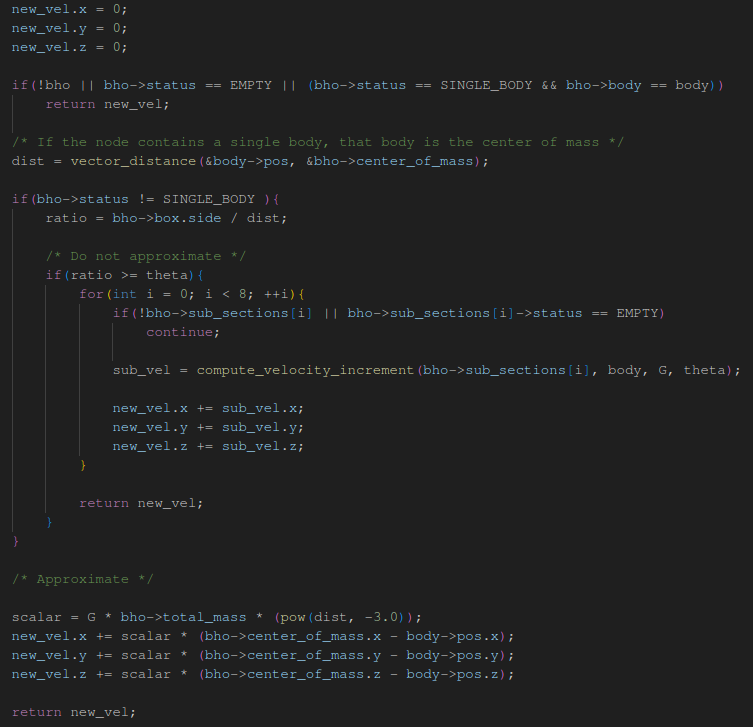
\includegraphics[width=\textwidth]{images/velocities.png}
        \caption{Screenshot del frammento di codice della funzione \texttt{compute\_velocity\_increment()} presente in \texttt{bh\_octree\_1.c}}
        \label{fig:velocities}
    \end{figure}

    \newpage

    Una volta definite quelle che sono le funzioni principali, l'intero algoritmo può essere ridotto all'applicazione in sequenza di suddette \textbf{tre procedure} ad ogni passo della simulazione, \textbf{distruggendo} l'albero dell'iterazione precedente, \textbf{ricalcolando} un nuovo albero tramite le nuove posizioni dei corpi e infine \textbf{computando} le nuove posizioni.

    \begin{figure}[H]
        \centering
        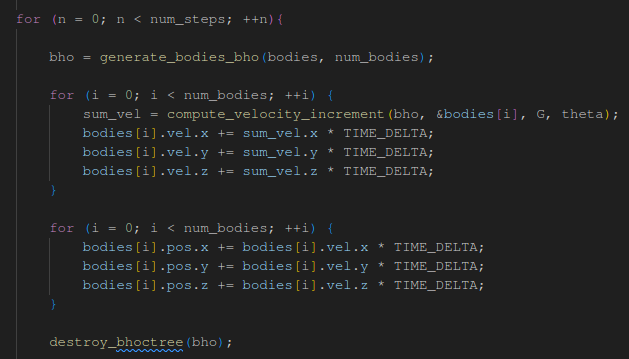
\includegraphics[width=\textwidth]{images/seq_bh_1.png}
        \caption{Screenshot del frammento di codice di interesse di \texttt{seq\_bh\_1.c}}
        \label{fig:seq_bh_1}
    \end{figure}

    \begin{figure}[H]
        \centering
        
        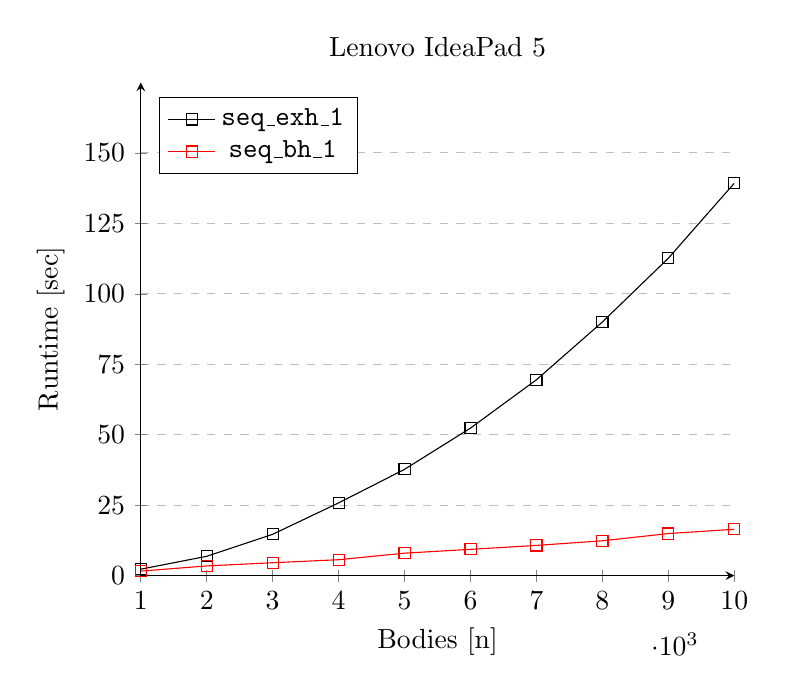
\begin{tikzpicture}
            \begin{axis}[
                axis lines = center,
                hide obscured x ticks=false,
                hide obscured y ticks=false,
                xlabel={Bodies [n]},
                ylabel={Runtime [sec]},
                ylabel near ticks,
                xlabel near ticks,
                xmin=1000, xmax=10000,
                ymin=0, ymax=175,
                xtick={1000, 2000, 3000, 4000, 5000, 6000, 7000, 8000, 9000, 10000},
                ytick={0, 25, 50, 75, 100, 125, 150},
                legend pos=north west,
                ymajorgrids=true,
                grid style=dashed,
                scaled x ticks= base 10:-3,
                scale=1.1,
                title=Lenovo IdeaPad 5
            ]
            
            \addplot[
                color=black,
                mark=square,
                ]
                coordinates {
                (1000, 2.29056454)
                (2000, 6.86578417)
                (3000, 14.67731190)
                (4000, 25.80976057)
                (5000, 37.72510433)
                (6000, 52.36848545)
                (7000, 69.51298285)
                (8000, 90.02810717)
                (9000, 112.65391874)
                (10000, 139.26667118)
                };

            \addplot[
                color=red,
                mark=square,
                ]
                coordinates {
                (1000, 1.605787754)
                (2000, 3.451525211)
                (3000, 4.584950924)
                (4000, 5.650474072)
                (5000, 7.979434967)
                (6000, 9.333063602)
                (7000, 10.727799892)
                (8000, 12.363978386)
                (9000, 14.939029694)
                (10000, 16.456793785)
                };

            \legend{\texttt{seq\_exh\_1},\texttt{seq\_bh\_1} }
            \end{axis}
        \end{tikzpicture}

        \quad 
        
        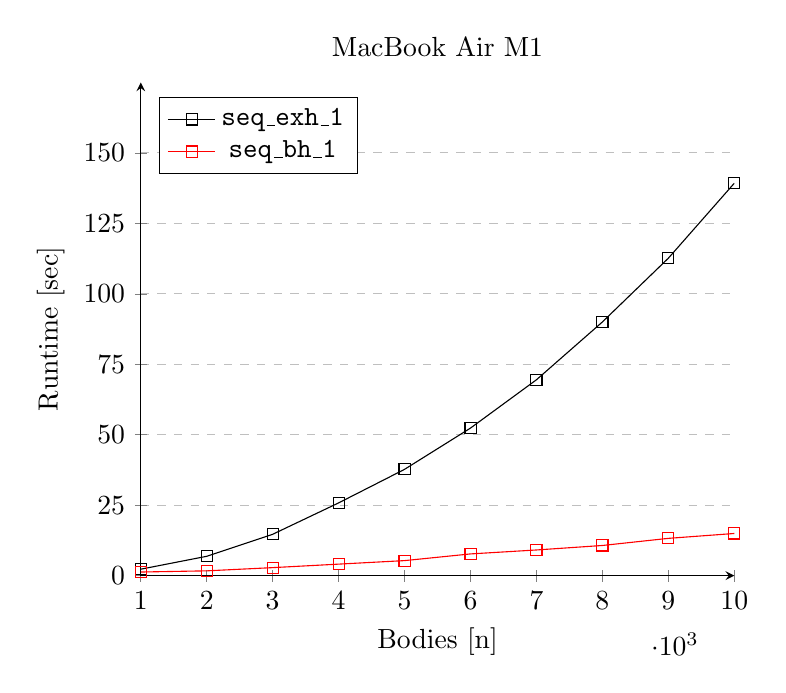
\begin{tikzpicture}
            \begin{axis}[
                axis lines = center,
                hide obscured x ticks=false,
                hide obscured y ticks=false,
                xlabel={Bodies [n]},
                ylabel={Runtime [sec]},
                ylabel near ticks,
                xlabel near ticks,
                xmin=1000, xmax=10000,
                ymin=0, ymax=175,
                xtick={1000, 2000, 3000, 4000, 5000, 6000, 7000, 8000, 9000, 10000},
                ytick={0, 25, 50, 75, 100, 125, 150},
                legend pos=north west,
                ymajorgrids=true,
                grid style=dashed,
                scaled x ticks= base 10:-3,
                scale=1.1,
                title=MacBook Air M1
            ]
            
            \addplot[
                color=black,
                mark=square,
                ]
                coordinates {
                (1000, 2.29056454)
                (2000, 6.86578417)
                (3000, 14.67731190)
                (4000, 25.80976057)
                (5000, 37.72510433)
                (6000, 52.36848545)
                (7000, 69.51298285)
                (8000, 90.02810717)
                (9000, 112.65391874)
                (10000, 139.26667118)
                };

            \addplot[
                color=red,
                mark=square,
                ]
                coordinates {
                (1000, 1.285310268)
                (2000, 1.704091549)
                (3000, 2.841899395)
                (4000, 4.086709499)
                (5000, 5.334965229)
                (6000, 7.708571911)
                (7000, 9.111736298)
                (8000, 10.704897881)
                (9000, 13.231217384)
                (10000, 14.963076115)
                };

            \legend{\texttt{seq\_exh\_1},\texttt{seq\_bh\_1} }
            \end{axis}
        \end{tikzpicture}

        \caption{Confronto delle performance di \texttt{seq\_exh\_1} e \texttt{seq\_bh\_1} con $\theta = 0.5$ su 100 passi di simulazione da 1000 a 10000 corpi. I numeri tra parentesi nella legenda del grafico indicano il numero di thread attivi}
        \label{fig:seq_1_bh_graph}
    \end{figure}

    \newpage

    \subsection{Ottimizzazioni della struttura dati}

    Nella versione \texttt{seq\_bh\_1.c}, potrebbe verificarsi che, a seguito dell'aggiorna-mento della sua posizione, un corpo \textbf{esca fuori} dal \textit{bounding box} del proprio nodo. In tal caso, risulta necessario che l'albero venga \textbf{distrutto} e \textbf{ricalcolato} al fine di poter aggiornare dove siano situati i corpi al suo interno.

    Tuttavia, tale operazione richiede la deallocazione e riallocazione dell'intero albero ad ogni passo della simulazione, generando un elevato rallentamento del programma, senza contare l'aggiuntivo rallentamento dato dal ricalcolo dell'intero albero, il quale spesso risulta \textit{non necessario} nel caso in cui nessun corpo sia uscito dal \textit{bounding box} del proprio nodo.

    Di conseguenza, è necessario ottimizzare l'intera struttura dati in modo che essa possa essere \textbf{aggiornata} senza essere interamente ricalcolata. Per raggiungere tale obiettivo, viene utilizzato un array di appoggio \texttt{leaves}, il quale memorizza per ogni corpo il puntatore al nodo foglia in cui è situato il corpo stesso. Tramite tale array aggiuntivo, è possibile definire la seguente procedura di aggiornamento:
    \begin{enumerate}
        \item Dato il corpo $b_i$, viene \textbf{verificato} se tale corpo sia uscito al di fuori del \textit{bounding box} del proprio nodo foglia
        \item Se ciò risulta falso, il controllo procede con il prossimo corpo
        \item Se cià risulta vero, l'albero viene percorso \textbf{dal basso verso l'alto} a partire dalla foglia contenente il nodo, procedendo finché non viene trovato un nodo sul cammino dalla foglia alla radice il cui \textit{bounding box} \textbf{contenga ancora il corpo}. Una volta trovato tale nodo, viene effettuato l'\textbf{inserimento} del corpo in tale nodo.
        \item In particolare, se neanche il \textit{bounding box} della radice dell'albero contiene il corpo, dunque se il corpo è uscito fuori da quello che precedentemente era lo spazio massimo, l'intero albero verrà \textbf{completamente rigenerato}, come nella versione \texttt{seq\_bh\_1}, espandendo così lo spazio massimo occupato dai corpi
    \end{enumerate}
    
    Per realizzare tale procedura efficientemente, è necessario che ogni nodo memorizzi anche un puntatore al proprio \textbf{nodo padre} e l'\textbf{indice del proprio sotto-settore} in cui tale nodo è situato all'interno dell'array dei figli del padre. Ad esempio, se il nodo $A$ corrisponde al figlio $4$ del proprio padre, allora tale indice verrà impostato su $4$. In tal modo, è possibile evitare di dover iterare su tutti i figli del padre in cerca di quale sia il sotto-settore in cui è situato il nodo stesso.

    \begin{figure}[H]
        \centering
        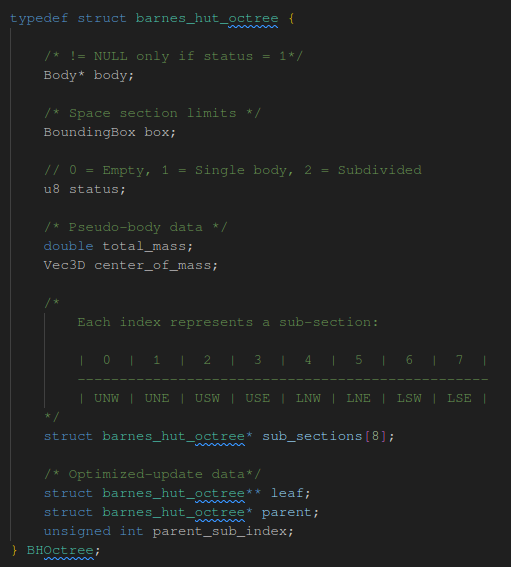
\includegraphics[width=\textwidth]{images/bhoctree_2.png}
        \caption{Screenshot del frammento di codice di interesse di \texttt{bh\_octree\_2.c}}
        \label{fig:bhoctree_2}
    \end{figure}

    \begin{figure}[H]
        \centering
        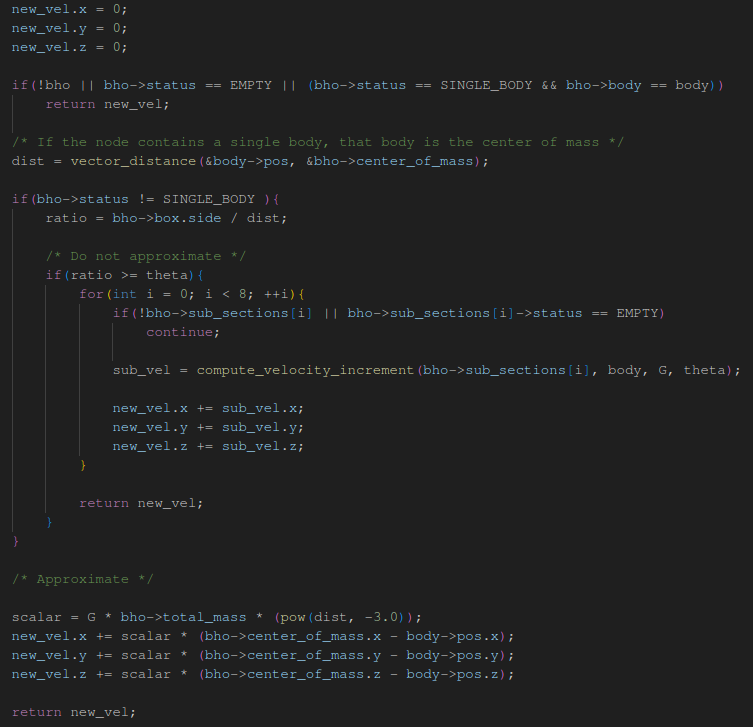
\includegraphics[width=\textwidth]{images/velocities.png}
        \caption{Screenshot del frammento di codice della funzione \texttt{update\_bodies\_bho()} presente in \texttt{bh\_octree\_2.c}}
        \label{fig:update_bodies}
    \end{figure}


    \begin{figure}[H]
        \centering
        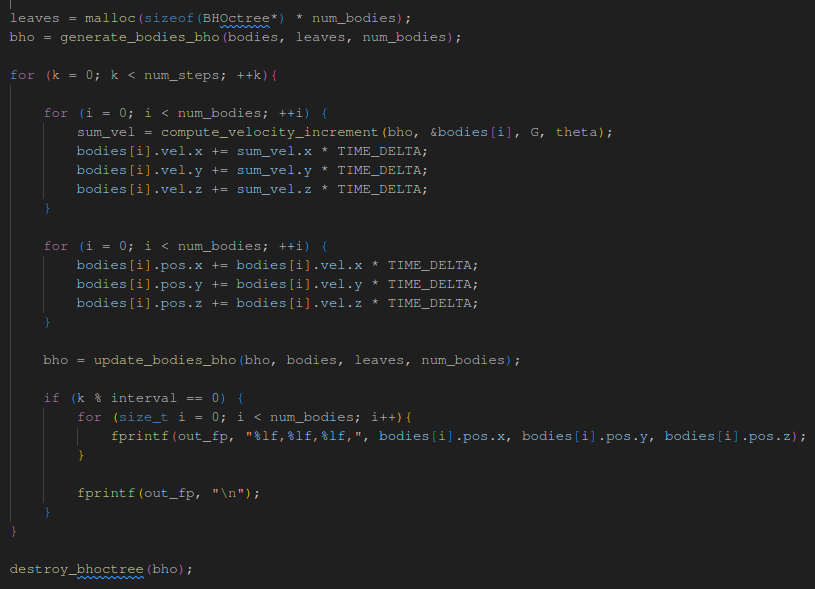
\includegraphics[width=\textwidth]{images/seq_bh_2.png}
        \caption{Screenshot del frammento di codice di interesse di \texttt{seq\_bh\_2.c}}
        \label{fig:seq_bh_2}
    \end{figure}

    Nel caso di molti corpi, tali parametri aggiuntivi incidono molto sulla \textbf{memoria totale occupata} dal programma nel suo intero poiché, dati $n$ corpi, l'albero può avere un massimo di $8n$ nodi istanziati contemporaneamente. Tuttavia, tale memoria aggiuntiva risulta trascurabile rispetto \textbf{netto miglioramento} delle performance del programma.

    \newpage

    \begin{figure}[H]
        \centering
        
        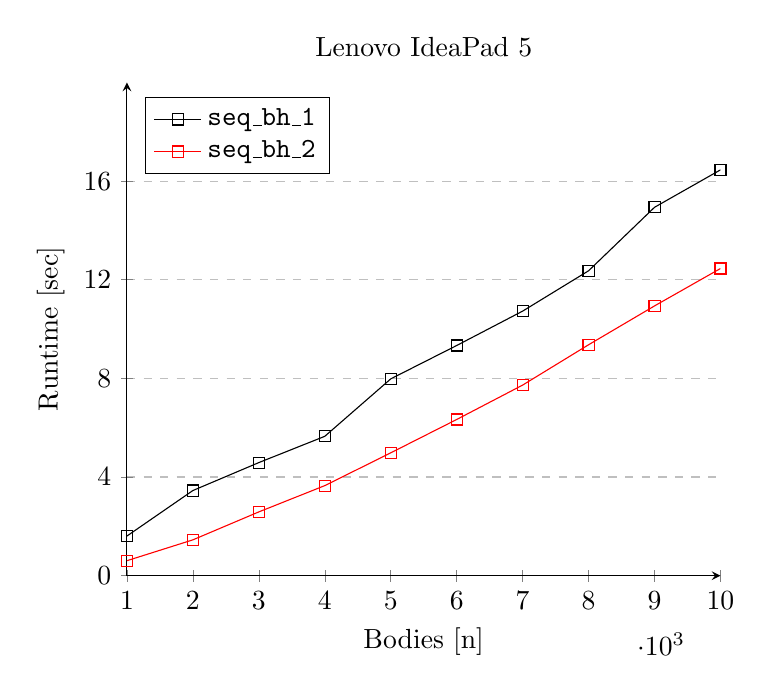
\begin{tikzpicture}
            \begin{axis}[
                axis lines = center,
                hide obscured x ticks=false,
                hide obscured y ticks=false,
                xlabel={Bodies [n]},
                ylabel={Runtime [sec]},
                ylabel near ticks,
                xlabel near ticks,
                xmin=1000, xmax=10000,
                ymin=0, ymax=20,
                xtick={1000, 2000, 3000, 4000, 5000, 6000, 7000, 8000, 9000, 10000},
                ytick={0, 4, 8, 12, 16},
                legend pos=north west,
                ymajorgrids=true,
                grid style=dashed,
                scaled x ticks= base 10:-3,
                scale=1.1,
                title=Lenovo IdeaPad 5
            ]
            
            \addplot[
                color=black,
                mark=square,
                ]
                coordinates {
                (1000, 1.605787754)
                (2000, 3.451525211)
                (3000, 4.584950924)
                (4000, 5.650474072)
                (5000, 7.979434967)
                (6000, 9.333063602)
                (7000, 10.727799892)
                (8000, 12.363978386)
                (9000, 14.939029694)
                (10000, 16.456793785)
                };

            \addplot[
                color=red,
                mark=square,
                ]
                coordinates {
                (1000, 0.605787754)
                (2000, 1.451525211)
                (3000, 2.584950924)
                (4000, 3.650474072)
                (5000, 4.979434967)
                (6000, 6.333063602)
                (7000, 7.727799892)
                (8000, 9.363978386)
                (9000, 10.939029694)
                (10000, 12.456793785)
                };

            \legend{\texttt{seq\_bh\_1},\texttt{seq\_bh\_2} }
            \end{axis}
        \end{tikzpicture}

        \quad 
        
        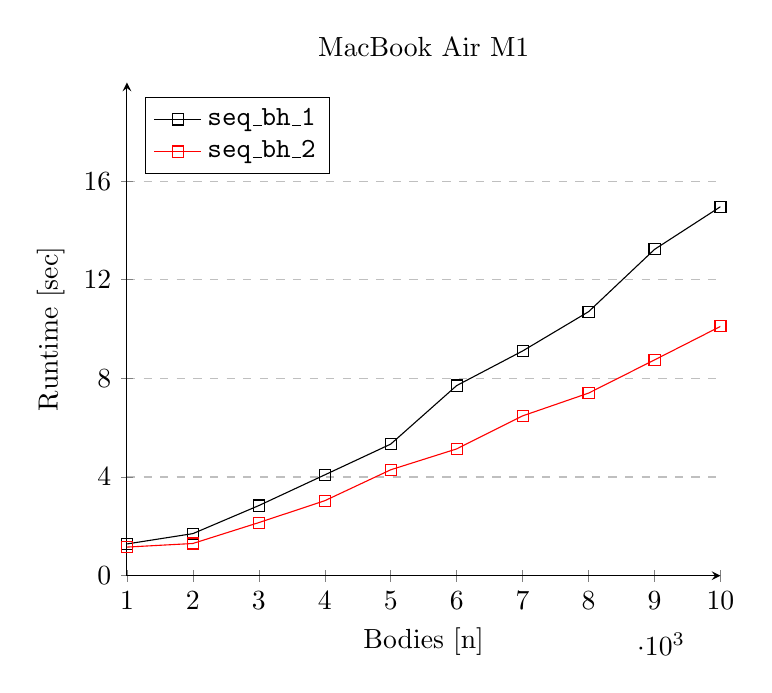
\begin{tikzpicture}
            \begin{axis}[
                axis lines = center,
                hide obscured x ticks=false,
                hide obscured y ticks=false,
                xlabel={Bodies [n]},
                ylabel={Runtime [sec]},
                ylabel near ticks,
                xlabel near ticks,
                xmin=1000, xmax=10000,
                ymin=0, ymax=20,
                xtick={1000, 2000, 3000, 4000, 5000, 6000, 7000, 8000, 9000, 10000},
                ytick={0, 4, 8, 12, 16},
                legend pos=north west,
                ymajorgrids=true,
                grid style=dashed,
                scaled x ticks= base 10:-3,
                scale=1.1,
                title=MacBook Air M1
            ]
            
            \addplot[
                color=black,
                mark=square,
                ]
                coordinates {
                (1000, 1.285310268)
                (2000, 1.704091549)
                (3000, 2.841899395)
                (4000, 4.086709499)
                (5000, 5.334965229)
                (6000, 7.708571911)
                (7000, 9.111736298)
                (8000, 10.704897881)
                (9000, 13.231217384)
                (10000, 14.963076115)
                };

            \addplot[
                color=red,
                mark=square,
                ]
                coordinates {
                (1000, 1.157885551)
                (2000, 1.304131985)
                (3000, 2.151301861)
                (4000, 3.038581848)
                (5000, 4.293384075)
                (6000, 5.140047073)
                (7000, 6.479253769)
                (8000, 7.403367519)
                (9000, 8.749234676)
                (10000, 10.109156609)
                };

            \legend{\texttt{seq\_bh\_1},\texttt{seq\_bh\_2}}
            \end{axis}
        \end{tikzpicture}

        \caption{Confronto delle performance di \texttt{seq\_bh\_1} e \texttt{seq\_bh\_2} con $\theta = 0.5$ su 100 passi di simulazione da 1000 a 10000 corpi. I numeri tra parentesi nella legenda del grafico indicano il numero di thread attivi}
        \label{fig:seq_2_bh_graph}
    \end{figure}

    \newpage

    \section{Parallelizzazione tramite OpenMP}

    \subsection{Analisi, limitazioni riscontrate e implementazione}

    Come per l'implementazione esaustiva, in particolare la versione \texttt{omp\_exh\_3}, il modo più diretto per poter parallelizzare l'algoritmo tramite OpenMP risulta essere tramite la \textbf{suddivisione a priori} dei corpi con cui i thread vanno a calcolare le varie interazioni.
    
    Tuttavia, a differenza dell'implementazione esaustiva, l'algoritmo di Barnes-Hut presenta una problematica aggiuntiva, ossia la \textbf{gestione dell'albero}: trattandosi di una struttura dati condivisa, risulta evidente pensare a problematiche relative all'\textbf{inserimento simultaneo dei nodi}, sia durante la creazione che durante l'aggiornamento.

    Per gestire tale problema, sono state considerate le seguenti soluzioni:

    \begin{enumerate}
        \item Implementare un \textbf{lock sulla radice} dell'albero, in modo che solo un thread per volta possa accedere all'intera struttura dati.
                
        \item Implementare un \textbf{lock su ogni nodo} dell'albero, in modo che solo un thread per volta possa accedere al nodo stesso
        
        \item Implementare un \textbf{optimistic locking} prima di effettuare modifiche ai nodi durante un inserimento

        \item Far sì che \textbf{solo un processo} si occupi di generare ed aggiornare l'albero mentre tutti gli altri attendono
    \end{enumerate}

    Dopo un'attenta analisi e prove di implementazione, è stato scelto di implementare l'\textbf{ultima soluzione}, in quanto le altre sono state ritenute come particolarmente \textbf{inefficienti} per i seguenti motivi:

    \begin{enumerate}
        \item Utilizzando un \textbf{lock sulla radice}, ogni thread dovrebbe attendere che il thread precedente termini tutti i propri inserimenti, rendendo difatti l'intera operazione del tutto identica all'ultima soluzione, tuttavia con un overhead aggiunto dovuto alla coordinazione tra i processi e alla gestione del lock
        \item Utilizzando un \textbf{lock su ogni nodo}, le performance di ogni operazione verrebbero drasticamente peggiorate in quanto ogni inserimento può propagarsi sull'intero albero, implicando che ogni inserimento debba richiedere e cedere continuamente il lock di ogni nodo attraversato nel cammino percorso
        \item Utilizzando l'\textbf{optimistic locking}, le performance di ogni operazione verrebbero drasticamente peggiorate in quanto ogni inserimento può generare modifiche a catena sui vari nodi attraversati, implicando che sia necessario effettuare la doppia scansione prevista dall'optimistic locking per ognuna di tali modifiche, rendendo il costo di un singolo inserimento pari a $O(n^2)$  
    \end{enumerate}

    \begin{figure}[H]
        \centering
        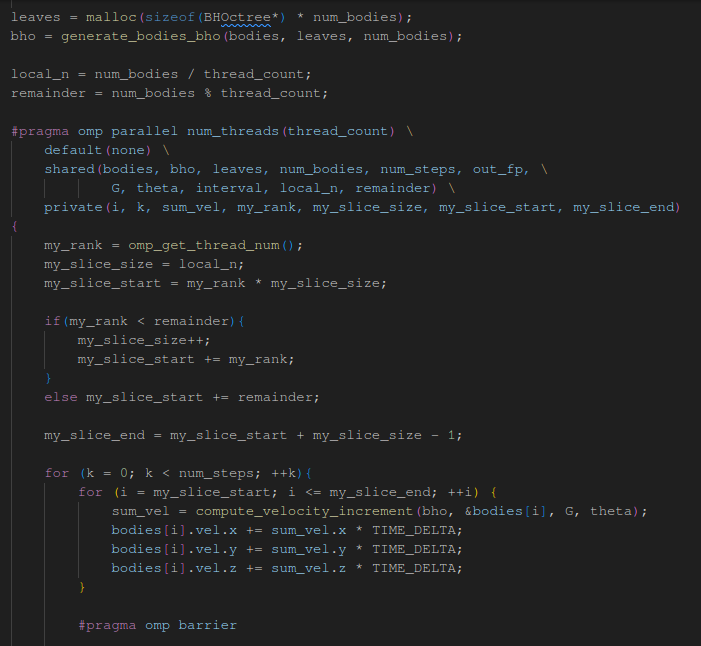
\includegraphics[width=\textwidth]{images/omp_bh_1.png}
    \end{figure}
    \begin{figure}[H]
        \centering
        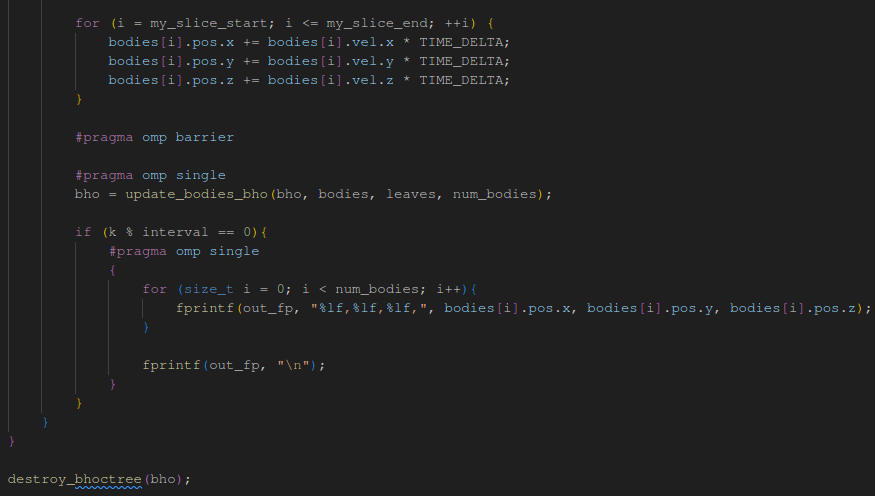
\includegraphics[width=\textwidth]{images/omp_bh_2.png}
        \caption{Screenshot del frammento di codice di interesse di \texttt{omp\_bh.c}}
        \label{fig:omp_bh}
    \end{figure}

    \begin{figure}[H]
        \centering
        
        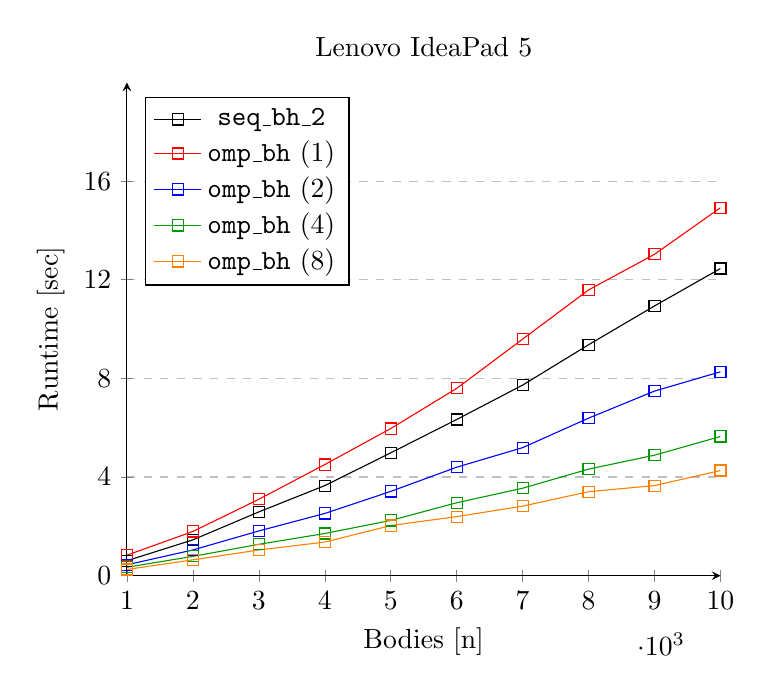
\begin{tikzpicture}
            \begin{axis}[
                axis lines = center,
                hide obscured x ticks=false,
                hide obscured y ticks=false,
                xlabel={Bodies [n]},
                ylabel={Runtime [sec]},
                ylabel near ticks,
                xlabel near ticks,
                xmin=1000, xmax=10000,
                ymin=0, ymax=20,
                xtick={1000, 2000, 3000, 4000, 5000, 6000, 7000, 8000, 9000, 10000},
                ytick={0, 4, 8, 12, 16},
                legend pos=north west,
                ymajorgrids=true,
                grid style=dashed,
                scaled x ticks= base 10:-3,
                scale=1.1,
                title=Lenovo IdeaPad 5
            ]
            
            \addplot[
                color=black,
                mark=square,
                ]
                coordinates {
                (1000, 0.605787754)
                (2000, 1.451525211)
                (3000, 2.584950924)
                (4000, 3.650474072)
                (5000, 4.979434967)
                (6000, 6.333063602)
                (7000, 7.727799892)
                (8000, 9.363978386)
                (9000, 10.939029694)
                (10000, 12.456793785)
                };

            \addplot[
                color=red,
                mark=square,
                ]
                coordinates {
                (1000, 0.829593658)
                (2000, 1.791427135)
                (3000, 3.095758438)
                (4000, 4.504912376)
                (5000, 5.965313911)
                (6000, 7.593463421)
                (7000, 9.591652870)
                (8000, 11.588360310)
                (9000, 13.033086300)
                (10000, 14.921123028)
                };
            
            \addplot[
                color=blue,
                mark=square,
                ]
                coordinates {
                (1000, 0.440105915)
                (2000, 1.041773319)
                (3000, 1.812405109)
                (4000, 2.521707058)
                (5000, 3.416090012)
                (6000, 4.398133278)
                (7000, 5.190513134)
                (8000, 6.387612343)
                (9000, 7.484739780)
                (10000, 8.269041061)
                };

            \addplot[
                color=green!60!black,
                mark=square,
                ]
                coordinates {
                (1000, 0.342028141)
                (2000, 0.781634808)
                (3000, 1.270354748)
                (4000, 1.708938122)
                (5000, 2.238661766)
                (6000, 2.956010342)
                (7000, 3.545292854)
                (8000, 4.320281982)
                (9000, 4.885052204)
                (10000, 5.644170761)
                };
            
            \addplot[
                color=orange,
                mark=square,
                ]
                coordinates {
                (1000, 0.249574184)
                (2000, 0.641079426)
                (3000, 1.039895058)
                (4000, 1.361323833)
                (5000, 2.031156063)
                (6000, 2.393718719)
                (7000, 2.818753242)
                (8000, 3.404787064)
                (9000, 3.652179718)
                (10000, 4.263443470)
                };

            \legend{\texttt{seq\_bh\_2},\texttt{omp\_bh} (1), \texttt{omp\_bh} (2), \texttt{omp\_bh} (4), \texttt{omp\_bh} (8), }
            \end{axis}
        \end{tikzpicture}

        \quad 
        
        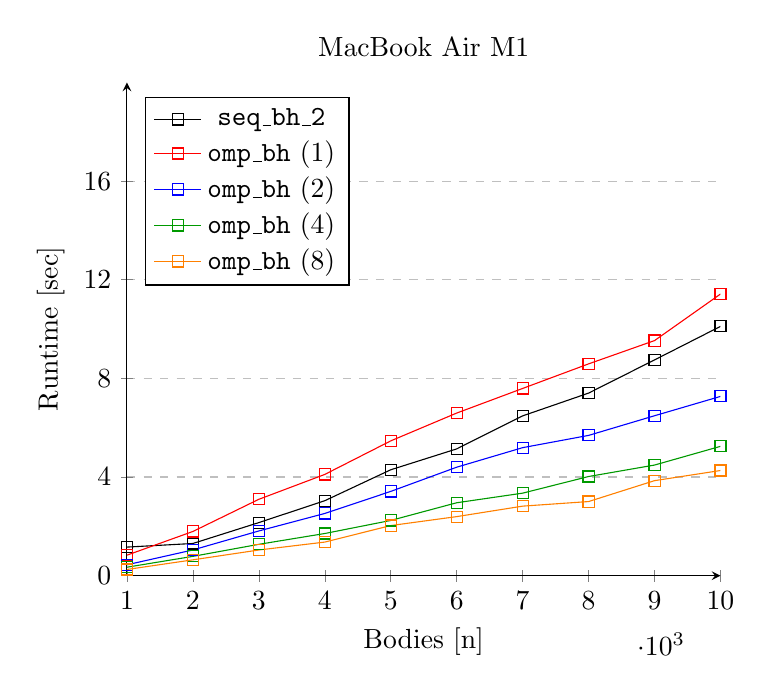
\begin{tikzpicture}
            \begin{axis}[
                axis lines = center,
                hide obscured x ticks=false,
                hide obscured y ticks=false,
                xlabel={Bodies [n]},
                ylabel={Runtime [sec]},
                ylabel near ticks,
                xlabel near ticks,
                xmin=1000, xmax=10000,
                ymin=0, ymax=20,
                xtick={1000, 2000, 3000, 4000, 5000, 6000, 7000, 8000, 9000, 10000},
                ytick={0, 4, 8, 12, 16},
                legend pos=north west,
                ymajorgrids=true,
                grid style=dashed,
                scaled x ticks= base 10:-3,
                scale=1.1,
                title=MacBook Air M1
            ]
                
            \addplot[
                color=black,
                mark=square,
                ]
                coordinates {
                (1000, 1.157885551)
                (2000, 1.304131985)
                (3000, 2.151301861)
                (4000, 3.038581848)
                (5000, 4.293384075)
                (6000, 5.140047073)
                (7000, 6.479253769)
                (8000, 7.403367519)
                (9000, 8.749234676)
                (10000, 10.109156609)
                };

            \addplot[
                color=red,
                mark=square,
                ]
                coordinates {
                (1000, 0.829593658)
                (2000, 1.791427135)
                (3000, 3.095758438)
                (4000, 4.104912376)
                (5000, 5.465313911)
                (6000, 6.593463421)
                (7000, 7.591652870)
                (8000, 8.588360310)
                (9000, 9.533086300)
                (10000, 11.421123028)
                };
            
            \addplot[
                color=blue,
                mark=square,
                ]
                coordinates {
                (1000, 0.440105915)
                (2000, 1.041773319)
                (3000, 1.812405109)
                (4000, 2.521707058)
                (5000, 3.416090012)
                (6000, 4.398133278)
                (7000, 5.190513134)
                (8000, 5.687612343)
                (9000, 6.484739780)
                (10000, 7.269041061)
                };

            \addplot[
                color=green!60!black,
                mark=square,
                ]
                coordinates {
                (1000, 0.342028141)
                (2000, 0.781634808)
                (3000, 1.270354748)
                (4000, 1.708938122)
                (5000, 2.238661766)
                (6000, 2.956010342)
                (7000, 3.345292854)
                (8000, 4.020281982)
                (9000, 4.485052204)
                (10000, 5.244170761)
                };
            
            \addplot[
                color=orange,
                mark=square,
                ]
                coordinates {
                (1000, 0.249574184)
                (2000, 0.641079426)
                (3000, 1.039895058)
                (4000, 1.361323833)
                (5000, 2.031156063)
                (6000, 2.393718719)
                (7000, 2.818753242)
                (8000, 3.004787064)
                (9000, 3.852179718)
                (10000, 4.263443470)
                };
    
            \legend{\texttt{seq\_bh\_2},\texttt{omp\_bh} (1), \texttt{omp\_bh} (2), \texttt{omp\_bh} (4), \texttt{omp\_bh} (8), }
            \end{axis}
        \end{tikzpicture}

        \caption{Confronto delle performance di \texttt{seq\_bh\_2} e \texttt{omp\_bh} con $\theta = 0.5$ su 100 passi di simulazione da 1000 a 10000 corpi. I numeri tra parentesi nella legenda del grafico indicano il numero di thread attivi}
        \label{fig:omp_bh_graph}
    \end{figure}

    \newpage

    \section{Parallelizzazione tramite MPI}
    
    \subsection{Analisi, limitazioni riscontrate e implementazione}
    
    Per parallelizzare l'algoritmo di Barnes-Hut utilizzando la libreria MPI si è optato per un approccio molto simile a quello della versione esaustiva analizzando cosa era sconveniente e limitante fra quello che era possibile parallelizzare:
    \begin{enumerate}
        \item Creazione e aggiornamento dell'albero
        \item Calcolo della velocità di ogni corpo
        \item Corpi da calcolare
    \end{enumerate}

    Un modo per parallelizzare la \textbf{creazione e l'aggiornamento} dell'albero sarebbe potuto essere quello di distribuire tra i processi \textbf{branch} diversi dell'albero per fare in modo che ognuno calcolasse la nuova disposizione dei nodi. Data però la natura sbilanciata dell'albero si avrebbero dei rami ricchi di nodi ed altri molto meno, dunque si avrebbero molti processi in wait che aspettano i processi più lenti per condividere la propria parte di albero ed eseguire il \textbf{mounting} dell'albero completo.
    In oltre ci sarebbe l'overhead aggiunto dalla divisione dei nodi e dei branch e soprattutto dalle comunicazioni aggiuntive necessarie. Dunque si è optato per lasciare che ogni processo modifichi per intero il proprio albero. 
    
    Si è scelto di parallelizzare solo sul numero di corpi di cui calcolare la posizione per ridurre al minimo l'overhead delle molteplici comunicazioni che sono limitate, come per la versione esaustiva, alle nuove posizioni calcolate. Ogni processo costruisce dunque il proprio albero e lo aggiorna con i valori delle posizioni condivise. 

    \begin{figure}[H]
        \centering
        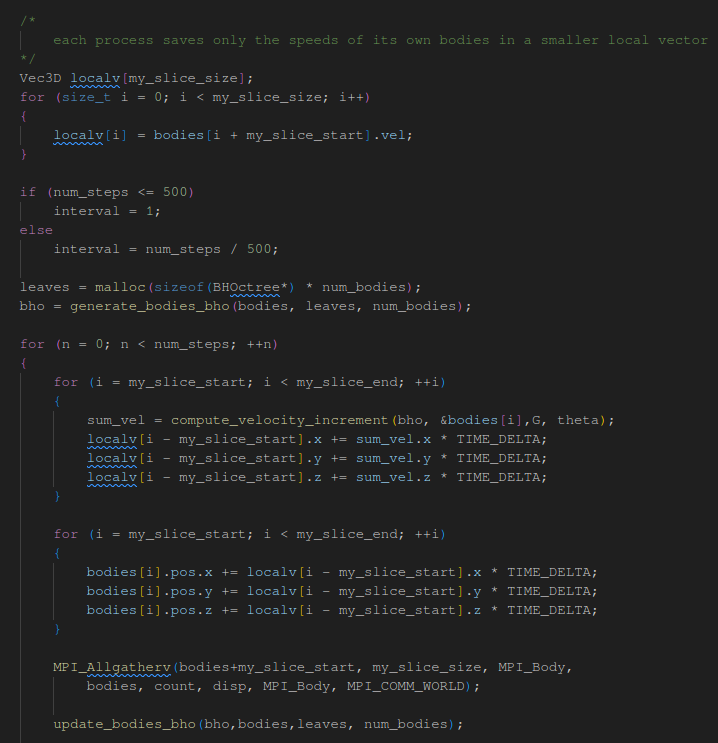
\includegraphics[width=\textwidth]{images/mpi_bh.png}
        \caption{Screenshot del frammento di codice di interesse di \texttt{mpi\_bh.c}}
        \label{fig:mpi_bh}
    \end{figure}


    \begin{figure}[H]
        \centering
        
        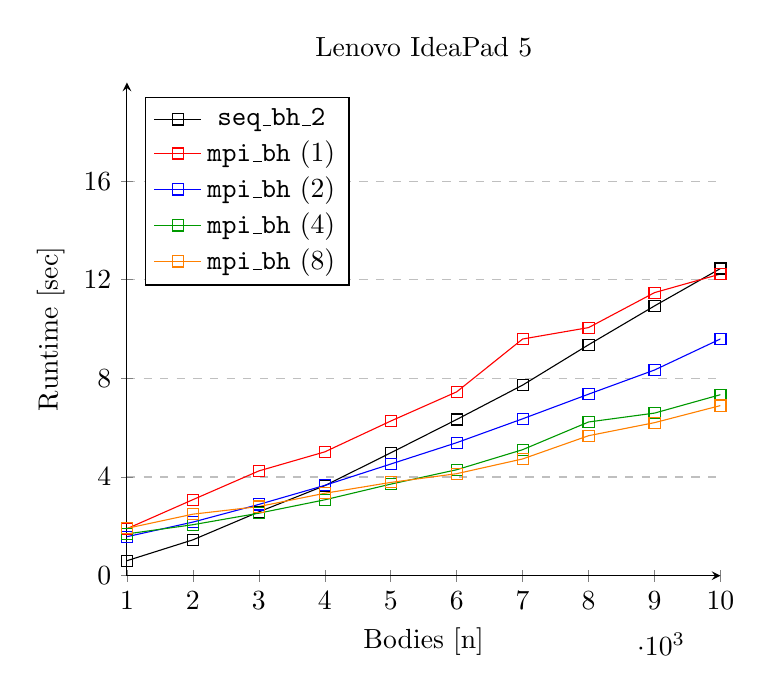
\begin{tikzpicture}
            \begin{axis}[
                axis lines = center,
                hide obscured x ticks=false,
                hide obscured y ticks=false,
                xlabel={Bodies [n]},
                ylabel={Runtime [sec]},
                ylabel near ticks,
                xlabel near ticks,
                xmin=1000, xmax=10000,
                ymin=0, ymax=20,
                xtick={1000, 2000, 3000, 4000, 5000, 6000, 7000, 8000, 9000, 10000},
                ytick={0, 4, 8, 12, 16},
                legend pos=north west,
                ymajorgrids=true,
                grid style=dashed,
                scaled x ticks= base 10:-3,
                scale=1.1,
                title=Lenovo IdeaPad 5
            ]
            
            \addplot[
                color=black,
                mark=square,
                ]
                coordinates {
                (1000, 0.605787754)
                (2000, 1.451525211)
                (3000, 2.584950924)
                (4000, 3.650474072)
                (5000, 4.979434967)
                (6000, 6.333063602)
                (7000, 7.727799892)
                (8000, 9.363978386)
                (9000, 10.939029694)
                (10000, 12.456793785)
                };

            \addplot[
                color=red,
                mark=square,
                ]
                coordinates {
                (1000, 1.902263165)
                (2000, 3.081031799)
                (3000, 4.246270657)
                (4000, 5.019849777)
                (5000, 6.269229412)
                (6000, 7.453901768)
                (7000, 9.596959877)
                (8000, 10.059731960)
                (9000, 11.478220940)
                (10000, 12.233047009)
                };
            
            \addplot[
                color=blue,
                mark=square,
                ]
                coordinates {
                (1000, 1.579219818)
                (2000, 2.171581268)
                (3000, 2.887826443)
                (4000, 3.660267830)
                (5000, 4.525997639)
                (6000, 5.392573833)
                (7000, 6.360850334)
                (8000, 7.359762669)
                (9000, 8.339801311)
                (10000, 9.599754333)
                };

            \addplot[
                color=green!60!black,
                mark=square,
                ]
                coordinates {
                (1000, 1.691954136)
                (2000, 2.065265656)
                (3000, 2.532935619)
                (4000, 3.075152874)
                (5000, 3.711215496)
                (6000, 4.295423508)
                (7000, 5.108428955)
                (8000, 6.231879234)
                (9000, 6.592075348)
                (10000, 7.339652538)
                };
            
            \addplot[
                color=orange,
                mark=square,
                ]
                coordinates {
                (1000, 1.919260025)
                (2000, 2.492624283)
                (3000, 2.802191734)
                (4000, 3.340042591)
                (5000, 3.781106949)
                (6000, 4.134671688)
                (7000, 4.732976437)
                (8000, 5.675232887)
                (9000, 6.205016136)
                (10000, 6.897924423)
                };

            \legend{\texttt{seq\_bh\_2},\texttt{mpi\_bh} (1), \texttt{mpi\_bh} (2), \texttt{mpi\_bh} (4), \texttt{mpi\_bh} (8), }
            \end{axis}
        \end{tikzpicture}

        \quad 
        
        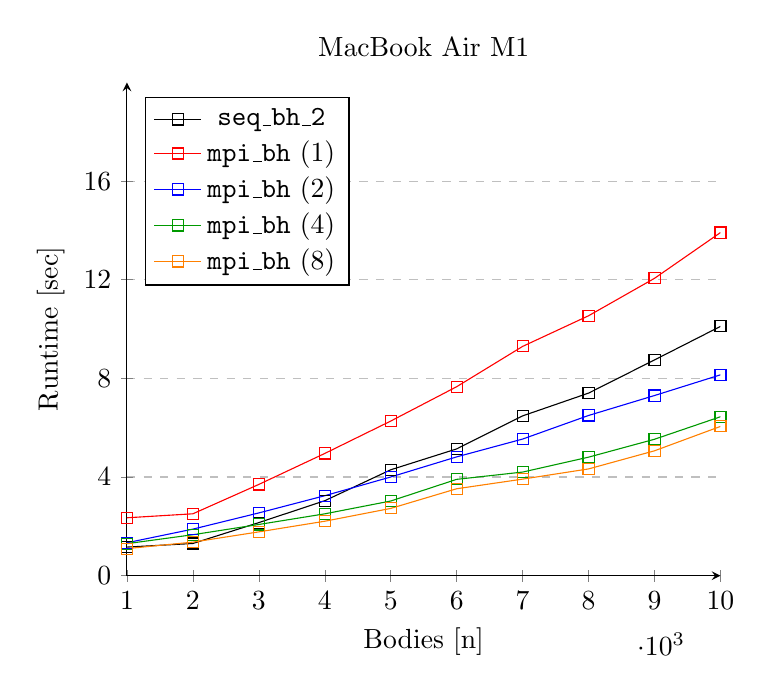
\begin{tikzpicture}
            \begin{axis}[
                axis lines = center,
                hide obscured x ticks=false,
                hide obscured y ticks=false,
                xlabel={Bodies [n]},
                ylabel={Runtime [sec]},
                ylabel near ticks,
                xlabel near ticks,
                xmin=1000, xmax=10000,
                ymin=0, ymax=20,
                xtick={1000, 2000, 3000, 4000, 5000, 6000, 7000, 8000, 9000, 10000},
                ytick={0, 4, 8, 12, 16},
                legend pos=north west,
                ymajorgrids=true,
                grid style=dashed,
                scaled x ticks= base 10:-3,
                scale=1.1,
                title=MacBook Air M1
            ]
                
            \addplot[
                color=black,
                mark=square,
                ]
                coordinates {
                (1000, 1.157885551)
                (2000, 1.304131985)
                (3000, 2.151301861)
                (4000, 3.038581848)
                (5000, 4.293384075)
                (6000, 5.140047073)
                (7000, 6.479253769)
                (8000, 7.403367519)
                (9000, 8.749234676)
                (10000, 10.109156609)
                };

            \addplot[
                color=red,
                mark=square,
                ]
                coordinates {
                (1000, 2.346283913)
                (2000, 2.508275509)
                (3000, 3.699564457)
                (4000, 4.955613613)
                (5000, 6.269229412)
                (6000, 7.662425518)
                (7000, 9.296959877)
                (8000, 10.540153503)
                (9000, 12.058612347)
                (10000, 13.914565563)
                };
            
            \addplot[
                color=blue,
                mark=square,
                ]
                coordinates {
                (1000, 1.334253788)
                (2000, 1.886823177)
                (3000, 2.543531418)
                (4000, 3.241585732)
                (5000, 4.001407623)
                (6000, 4.816792011)
                (7000, 5.539497375)
                (8000, 6.496120930)
                (9000, 7.304877758)
                (10000, 8.144491196)
                };

            \addplot[
                color=green!60!black,
                mark=square,
                ]
                coordinates {
                (1000, 1.296394825)
                (2000, 1.659616470)
                (3000, 2.075272083)
                (4000, 2.506777763)
                (5000, 3.026667595)
                (6000, 3.905524731)
                (7000, 4.200504780)
                (8000, 4.805781841)
                (9000, 5.531794548)
                (10000, 6.444715023)
                };
            
            \addplot[
                color=orange,
                mark=square,
                ]
                coordinates {
                (1000, 1.096394825)
                (2000, 1.359616470)
                (3000, 1.775272083)
                (4000, 2.206777763)
                (5000, 2.726667595)
                (6000, 3.524033070)
                (7000, 3.914837933)
                (8000, 4.328553009)
                (9000, 5.063516617)
                (10000, 6.052484035)
                };

            \legend{\texttt{seq\_bh\_2},\texttt{mpi\_bh} (1), \texttt{mpi\_bh} (2), \texttt{mpi\_bh} (4), \texttt{mpi\_bh} (8), }
            \end{axis}
        \end{tikzpicture}

        \caption{Confronto delle performance di \texttt{seq\_bh\_2} e \texttt{mpi\_bh} con $\theta = 0.5$ su 100 passi di simulazione da 1000 a 10000 corpi. I numeri tra parentesi nella legenda del grafico indicano il numero di thread attivi}
        \label{fig:mpi_bh_graph}
    \end{figure}


    \newpage

    \section{Analisi dello speed-up e dell'efficienza}

    Tramite i dati inerenti al runtime delle varie versioni parallelizzate e non mostrati nelle sezioni precedenti, consideriamo lo \textbf{speed-up} e l'\textbf{efficienza} ottenute da ognuna di tali versioni rispetto all'implementazione sequenziale \texttt{seq\_bh\_2} nel caso con 10000 corpi e $\theta = 0.5$.

    \begin{figure}[H]
        \centering

        \begin{tabular}{ l | c | c | c }
            \textbf{Programma} & \textbf{Runtime} & \textbf{Speed-up} & \textbf{Efficienza}\\
            \hline
            \texttt{seq\_bh\_2} & 12.456793785 & 1.000000000 & 1.00 \\
            \hline
            \texttt{omp\_bh (1)} & 14.921123028 & 0.834842911 & 0.83 \\
            \texttt{omp\_bh (2)} & 8.269041061 & 1.506437529 & 0.75 \\
            \texttt{omp\_bh (4)} & 5.644170761 & 2.207019297 & 0.55 \\
            \texttt{omp\_bh (8)} & 4.263443470 & 2.921768254 & 0.36 \\
            \hline
            \texttt{mpi\_bh (1)} & 12.233047009 & 1.018290355 & 1.01 \\
            \texttt{mpi\_bh (2)} & 9.599754333 & 1.297615892 & 0.64 \\
            \texttt{mpi\_bh (4)} & 7.339652538 & 1.697191212 & 0.42 \\
            \texttt{mpi\_bh (8)} & 6.897924423 & 1.805875655 & 0.22 \\
        \end{tabular}
        \caption{Statistiche per dispositivo Lenovo IdeaPad 5}
        \label{fig:stats_ip5_2}
    \end{figure}

    \begin{figure}[H]
        \centering

        \begin{tabular}{ l | c | c | c }
            \textbf{Programma} & \textbf{Runtime} & \textbf{Speed-up} & \textbf{Efficienza}\\
            \hline
            \texttt{seq\_bh\_2} & 10.109156609 & 1.000000000 & 1.00 \\
            \hline
            \texttt{omp\_bh (1)} & 11.421123028 & 0.885128072 & 0.88 \\
            \texttt{omp\_bh (2)} & 7.269041061 & 1.390713923 & 0.69 \\
            \texttt{omp\_bh (4)} & 5.244170761 & 1.927694019 & 0.48 \\
            \texttt{omp\_bh (8)} & 4.263443470 & 2.371124815 & 0.30 \\
            \hline
            \texttt{mpi\_bh (1)} & 13.914565563 & 0.726516151 & 0.72 \\
            \texttt{mpi\_bh (2)} & 8.144491196 & 1.241226292 & 0.62 \\
            \texttt{mpi\_bh (4)} & 6.444715023 & 1.568596373 & 0.39 \\
            \texttt{mpi\_bh (8)} & 6.052484035 & 1.670249199 & 0.21 \\
        \end{tabular}
        \caption{Statistiche per dispositivo MacBook Air M1}
        \label{fig:stats_m1_2}
    \end{figure}

    \newpage

    \chapter{Conclusioni}

    Come mostrato dalle analisi precedenti, entrambi i due algoritmi risultano \textit{sfavorevoli} all'uso della \textbf{memoria distribuita} per via della necessità di effettuare una comunicazione ad ogni passo della simulazione. L'overhead imposto da tali comunicazioni risulta trascurabile solo nel caso in cui vengano trasmesse enormi quantità di dati in una singola comunicazione.

    Viceversa, l'uso della \textbf{memoria condivisa} fornisce risultati più \textit{omogenei} tra loro. Tuttavia, anche tale modalità presenta le sue complicazioni, in particolare per quanto riguarda l'alta difficoltà nel \textbf{parallelizzare la struttura dati} utilizzata dall'algoritmo Barnes-Hut. Un'eventuale implementazione che sia in grado di parallelizzare correttamente tale struttura dati con l'introduzione di un minimo overhead per eventuali attese durante inserimenti simultanei porterebbe l'algoritmo ad aver performance più elevate.

    Per quanto riguarda l'analisi sullo \textit{speed-up} e l'\textit{efficienza}, essi risultano tendenzialmente massimi durante l'utilizzo di \textbf{4 processori} contemporaneamente. In particolare, tali statistiche risultano particolarmente elevate nelle varie implementazioni con \textbf{metodo esaustivo}. 

    \quad

    Il codice sorgente relativo a questo documento può essere trovato al seguente link: \href{https://github.com/Exyss/n-body-parallelization}{https://github.com/Exyss/n-body-parallelization}
\end{document}